\chapter{Introducción y motivación}

<<<<<<< HEAD

Toda observación de cualquier fenómeno astronómico, requiere de múltiples trabajos laboriosos y operaciones de control, para cada componente del observatorio. Ya sea la montura del telescopio (sección~\ref{montura}), la cámara CCD (sección~\ref{ccd}), el enfocador (sección~\ref{enfocadores}), la rueda de filtros (sección~\ref{filtros}) etc., asumiendo una pérdida de tiempo útil y el riesgo que se puedan producir errores humanos o accidentes, que pongan en peligro la noche de observación.


Muchas de las operaciones siguen patrones claros y tienen relación con el estado de un sensor o periférico, permitiendo definir rutinas automáticas que agilicen los trabajos inherentes a la observación. 

Un ejemplo claro puede ser la decisión de abrir o cerrar la cúpula en un momento dado en función de los datos proporcionados por la estación meteorológica (sección~\ref{estacion_meteorologica}).


En el mercado existen ya gran cantidad de recursos que se encargan de automatizar estas tareas, sin embargo, el acceso a estos recursos es caro y no todo aficionado a la astronomía puede permitírselo.  

Otro punto en contra de estas soluciones, es que suelen ser muy cerradas. Las compañías ofrecen muy pocos detalles técnicos (los justos para poder instalarlos e integrarlos), no permiten ninguna modificación y deben funcionar exactamente bajo la plataformas definidas, en la mayoría de los casos con el sistema operativo Windows. 

El presente proyecto se puede englobar dentro de las soluciones ``Internet of Things'' que hoy día están en una de las fases de expectativas más alta, como podemos observar en el \textit{Hype Cycle for Emerging Technologies} de Gartner \cite{hypeGartner} (figura~\ref{fig:gartner}).


\begin{figure}[h]
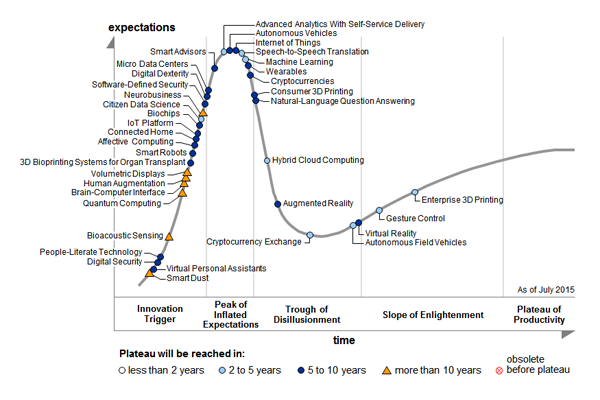
\includegraphics[width=1\linewidth]{../images/emergingGartner}
\caption[Hype Cycle for Emerging Technologies]{Hype Cycle for Emerging Technologies, 2015. \textbf{Fuente:}~\cite{hypeGartner}}
\label{fig:gartner}
\end{figure}


Para poner en contexto el proyecto, en las siguientes secciones se propone un recorrido por algunas de las ciencias, tecnologías y disciplinas que están involucradas en el desarrollo del presente TFG:

=======
\bigskip
Toda observación de cualquier fenómeno astronómico requiere de múltiples trabajos laboriosos y operaciones de control para cada componente del observatorio, ya sea la montura del telescopio, la cámara CCD, el enfocador, la rueda de filtros etc., asumiendo una pérdida de tiempo útil y un riesgo que se puedan producir errores humanos o accidentes, que pongan en peligro la noche de observación.

\bigskip
Muchas de las operaciones siguen patrones claros, y tienen relación con el estado de un sensor o periférico, por tanto podemos definir rutinas automáticas, 
que agilicen los trabajos inherentes a la observación. 

\bigskip
Un ejemplo claro puede ser la decisión de abrir o cerrar la cúpula en un momento dado en función de los datos proporcionados por la estación meteorológica, o la decisión de corregir el foco según el perfil de brillo obtenido para las estrellas presentes en las imágenes tomadas por la cámara CCD.

\bigskip
En el mercado existen ya gran cantidad de recursos que se encargan de automatizar las tareas antes citadas, sin embargo, el acceso a estos recursos es caro y no todo aficionado a la astronomía puede permitírselo.  Además el nivel de complejidad de algunos modelos complican su manejo y por tanto el disfrute en la observación.
Otro punto en contra de estas soluciones es que suelen ser muy cerradas, las compañías ofrecen muy pocos detalles tecnicos (los justos para poder instalarlos e integrarlos), no permiten ninguna modificación y deben funcionar exactamente bajo la plataformas definidas, en la mayoría de los cosas Windows. 

\newpage
\bigskip
Para poner en contexto el proyecto, se  propone un recorrido por algunos de las ciencias, tecnologías y disciplinas que están involucradas en el desarrollo del presente TFG.
>>>>>>> c9f08dfe66521d4f0dba18e652f93a6a37a333aa

\begin{itemize}

  \item {Astronomía}
<<<<<<< HEAD
%    \begin{itemize}
%    	\setlength\itemsep{0em}
% 	   \item{Clásica}
% 	   \item{Moderna}
% 	   \item{Actual}	 
% 	\end{itemize}

  \item {Instrumental astronómico}
%   \begin{itemize}
%   	\setlength\itemsep{0em}	
%     \item{Telescopios}
%     \item{Monturas robotizadas}
%     \item{Enfocadores}
%     \item{Cámara y CCD}
%     \item{Rueda portafiltros}
%     \item{Cúpulas y estaciones meteorológicas}
%       
%  \end{itemize}
  \item {Software astronómico}
  \item {Formato imágenes astronómicas}
  
  \item {Control remoto de observatorios}
%   \begin{itemize}
%   	\setlength\itemsep{0em}
%    	\item{ASCOM}
%    	\item{INDI}
%    	\item{Clientes remotos}
%   \end{itemize}
  
  \item {Hardware libre}
%    \begin{itemize}
%    	\setlength\itemsep{0em}
%      \item{Arduino}
%      \item{Raspberry Pi}
%    \end{itemize}
   
   \item {Enfocadores astronómicos: estado del arte}
=======
   \begin{itemize}
	   \item{Clásica}
	   \item{Moderan}
	   \item{Actual}	 
	\end{itemize}

  \item {Instrumental astronómico}
  \begin{itemize}	
    \item{Telescopios}
    \item{Monturas Robotizadas}
    \item{Enfocadores}
    \item{Cámara y CCD}
    \item{Rueda Portafiltros}
    \item{Cúpulas y estaciones meteorológicas}
      
  \end{itemize}
  
  \item {Hardware libre}
   \begin{itemize}
     \item{Arduino}
     \item{Raspberry Pi}
   \end{itemize}
   
  \item {Observatorios remotos}
   \begin{itemize}
     \item{ASCOM}
     \item{INDI}
     \item{Clientes remotos}
  \end{itemize}
  
  \item{Formato Imágenes}
  \item {Software procesamiento imagenes astronómicas}
>>>>>>> c9f08dfe66521d4f0dba18e652f93a6a37a333aa

\end{itemize}


\begin{figure}[h]
<<<<<<< HEAD
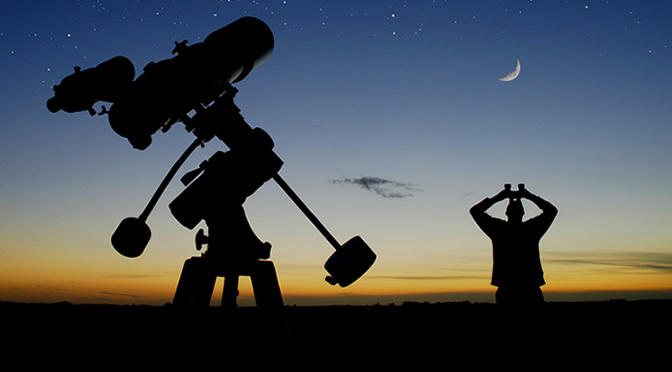
\includegraphics[width=1\linewidth]{../images/observatorio_amateur}
\caption[Observatorio Amateur]{\textbf{Astrónomo amateur} en plena observación, utilizando telescopio y prismáticos. \textbf{Fuente:} \cite{astrociencia}}
\label{fig:observatorio_amateur}
\end{figure}

=======
\centering
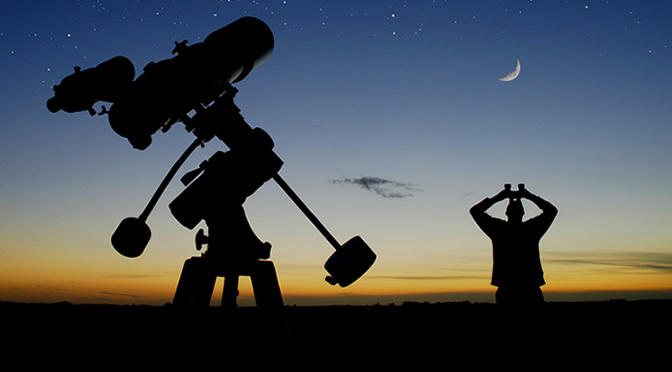
\includegraphics[width=0.7\linewidth]{../images/observatorio_amateur}
\caption[Observatorio Amateur]{\href{http://astrocienciasecu.blogspot.com.es/}{Observatorio Amateur}}
\label{fig:observatorio_amateur}
\end{figure}
\newpage
>>>>>>> c9f08dfe66521d4f0dba18e652f93a6a37a333aa

\section{La Astronomía}


Significa literalmente el estudio de las \textbf{leyes} que rigen los \textbf{astros} o cuerpos celestes, según su etimología griega y latina.

<<<<<<< HEAD

Se define más formalmente como \cite{astronomia}:

\begin{quote}``\textit{Ciencia que se ocupa del estudio de los cuerpos celestes del universo, incluidos los planetas y sus satélites, los cometas y meteoritos, las estrellas y la materia interestelar,
  los sistemas de materia oscura, estrellas, gas y polvo llamados galaxias y los cúmulos de galaxias; por lo que estudia sus movimientos y fenómenos ligados a ellos.}''
\end{quote}


Es una de las ciencia más remota por su impacto visual, emocional y su gran utilidad en la agricultura. Captó la atención de nuestros antepasados, motivándolos al estudio de los objetos del firmamento y su movimiento, fenómeno que muchas veces no conseguían explicar por completo, y por eso los llegaban a divinizar en múltiples culturas.


Por tanto la  astronomía es una ciencia antigua y moderna a la vez: Antigua porque se remonta prácticamente al origen de la humanidad; Moderna por proporcionar uno de los campos de estudio e investigación más avanzados.


Se trata de una ciencia donde aún perduran muchos interrogantes como por ejemplo, si existe vida fuera de la Tierra o si somos la única civilización inteligente \cite{astrociencia}.
=======
\bigskip
Se define más formalmente como:

\begin{quote}``\textit{Ciencia que se ocupa del estudio de los cuerpos celestes del universo, incluidos los planetas y sus satélites, los cometas y meteoritos, las estrellas y la materia interestelar,
  los sistemas de materia oscura, estrellas, gas y polvo llamados galaxias y los cúmulos de galaxias; por lo que estudia sus movimientos y fenómenos ligados a ellos.}''
\newline(\href{https://es.wikipedia.org/wiki/Astronom%C3%ADa}{Astronomia})
\end{quote}

\bigskip
Se puede afirmar que fue la ciencia más remota por su impacto visual, emocional y gran utilidad en la agricultura, por ello captó la atención de nuestros antepasados, motivandolos al estudio de los objetos suspendidos en el firmamento, fenómenos que muchas veces no conseguían explicar por completo, y por eso los llegaban a divinizar en múltiples culturas.

\bigskip
Por tanto la  astronomía es una ciencia antigua y moderna a la vez. \newline
Antigua porque se remonta prácticamente al origen de la humanidad.\newline
Moderna por proporcionar uno de los campos de estudio e investigación más avanzados.

\bigskip
Se trata por tanto de una ciencia cargada de múltiples misterios que a día de hoy se siguen manteniéndose, con muchos interrogante, como por ejemplo,  si existe vida fuera de la Tierra, o si somos la única civilización
inteligente.


\begin{figure}[b]
\centering
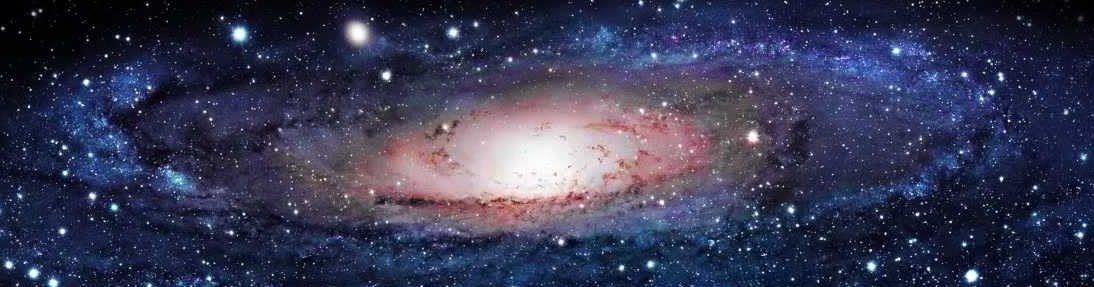
\includegraphics[width=0.9\linewidth]{../images/astrofooter}
\caption[Galaxia M88]{\href{https://commons.wikimedia.org/wiki/File:Messier_88_galaxy.jpg}{Galaxia M88}}
\label{fig:astrofooter}
\end{figure}
>>>>>>> c9f08dfe66521d4f0dba18e652f93a6a37a333aa


\subsection{Astronomía Antigua}

<<<<<<< HEAD
=======
\bigskip
Civilizaciones tan antiguas como la asiria, babilónica o  sumeria, ya comenzaron a transmitirnos los primeros conocimientos sobre el universo que conocemos gracias a la difusión realizada por la cultura griega.
>>>>>>> c9f08dfe66521d4f0dba18e652f93a6a37a333aa

Civilizaciones tan antiguas como la asiria, babilónica o sumeria, ya comenzaron a transmitirnos los primeros conocimientos sobre el universo que conocemos gracias a la difusión realizada por la cultura griega \cite{historiaAstronomia}.

<<<<<<< HEAD

Tienen especial importancia los conocimientos astronómicos de los egipcios, dado que para ellos el estudio del cielo y elaborar su \textbf{calendario egipcio} \cite{calendario_egipcio} les era de vital importancia, porque les permitía controlar los ciclos de la agricultura y prever la gran inundación del río Nilo, que sigue ciclos anuales.


En el Nuevo Mundo, los mayas llegaron a alcanzar importantes conocimientos de los cuerpos celestes y elaborando un calendario bastante preciso. 


Los incas se consideraban a sí mismos descendientes del Sol y los aztecas adoraban al dios \textbf{Huitzilopochtli}, símbolo del Sol que amanecía cada mañana para hacer la lucha con sus hermanas, las estrellas y así imponer su reinado diurno.


En el  siglo III a.C, el astrónomo griego \textbf{Aristarco de Samos}~\cite{Arist}, puso en duda todo el modelo geocéntrico griego y postuló que la Tierra gira en 24 horas y se traslada en torno al Sol en un año. Realizando también dibujos de las órbitas planetarias en el orden que ahora las conocemos.


\textbf{Pitágoras}~\cite{Pitagoras} en el siglo VI  a.C. ya tenia ideas sobre los movimientos de rotación  Terrestre y de traslación en torno al Sol, así como conocimiento de la esfericidad de la Tierra, Luna y Sol~\cite{AstroAnti}.

=======
\bigskip
Teniendo especial importancia los conocimientos astronómicos de los egipcios, dado para ellos el estudio del cielo y elaborar su 
(\href{https://es.wikipedia.org/wiki/Calendario_egipcio}{\textbf{calendario egipcio}} que les era de vital importancia, dado que permitía controlar los ciclos de la agricultura y prever la gran inundación del río Nilo, que sigue ciclos anuales.

\bigskip
En el Nuevo Mundo, los mayas llegaron a alcanzar importantes conocimientos de los cuerpos celestes y elaborando un calendario bastante preciso. 
\newline

\bigskip
Los incas se consideraban a sí mismos descendientes del Sol y los aztecas adoraban al dios \textbf{Huitzilopochtli}, símbolo del Sol
que amanecía cada mañana para hacer la lucha con sus hermanas, las estrellas y así imponer su reinado diurno.
\newline

\bigskip
Se presume que ya en el  siglo III a,C, el astrónomo griego \textbf{Aristarco de Samos} ~\cite{Arist} puso en duda todo el modelo geocéntrico griego y postuló que la Tierra gira en 24 horas y se traslada en torno al Sol en un año. Realizando también dibujos de las órbitas planetarias en el orden que ahora las conocemos.

\bigskip
\textbf{Pitágoras} ~\cite{Pitagoras} en el siglo VI  a.C. ya tenia ideas sobre los movimientos de rotación  Terrestre en torno a su eje, de traslación en torno al Sol y conocimiento de la esfericidad de la Tierra, Luna y So.  ~\cite{AstroAnti}.
>>>>>>> c9f08dfe66521d4f0dba18e652f93a6a37a333aa


\subsection{Astronomía Moderna}

<<<<<<< HEAD
=======
\bigskip
Se dice que la Astronomía moderna\cite{AstMod} inicia su desarrollo con Nicolás Copérnico (1473-1543)  quien el año de su muerte publica un trabajo de importancia capital, \textbf{De revolutionibus orbium caelestium}\cite{Copernico}.
>>>>>>> c9f08dfe66521d4f0dba18e652f93a6a37a333aa

La Astronomía moderna \cite{AstMod} inicia su desarrollo con \textbf{Nicolás Copérnico (1473-1543)} \cite{Copernico}, quien el año de su muerte publica su trabajo más importante \textbf{De revolutionibus orbium caelestium}.

<<<<<<< HEAD

Se mantiene que la Tierra tiene un doble movimiento: de rotación sobre ella misma, en 24 horas, y de revolución alrededor del Sol, en un año. También establece movimientos similares para los planetas y satélites.


Una figura muy importante es \textbf{Tycho Brahe (1546-1601)} \cite{Tycho} con  sus observaciones, facilitó a su discípulo \textbf{Johannes Kepler (1571-1630)} \cite{Kepler}, el descubrimiento de las famosas leyes que rigen el movimiento de los planetas, el abandono de las órbitas circulares y la ruptura definitiva con unos conceptos tradicionales que estaban profundamente arraigados. 



\textbf{Galileo Galilei (1564, 1642)} \cite{galileo} fue un astrónomo, filósofo, ingeniero, matemático y físico italiano. En 1609 construye su primer telescopio, motivado por el rumor de la existencia de un telescopio fabricado en Holanda. Su telescopio no deforma los objetos y es capaz de aumentarlos 6 veces. Tras muchas versiones consigue aumentar los objetos hasta 20 veces. Con su instrumento realiza numerosos descubrimientos de la morfología de la Luna y del universo en general.  
 


=======
\bigskip
Una aportación fundamental en el desarrollo de la nueva es debida a Tycho Brahe (1546-1601)\cite{Tycho} teniendo gran importancia sus observaciones, y  sentando las bases que facilitarían a su discípulo Johannes Kepler (1571-1630)\cite{Kepler}, el descubrimiento de las famosas leyes que rigen el movimiento, el abandono de las órbitas circulares y la ruptura definitiva con unos conceptos tradicionales que estaban profundamente arraigados. 

\bigskip
La publicación de los Principia en 1685 por Isaac Newton (1643-1727)\cite{Newton} marca uno de los puntos culminantes de la ciencia moderna, las leyes de Kepler quedan incluidas en un sistema físico que explica una serie de fenómenos naturales como las estaciones del año, las mareas, los movimientos de los astros, mediante un conjunto consistente de leyes de carácter general que podían ser probadas en un laboratorio.

\bigskip
En este punto Astronomía y Astrología inician caminos diferentes y desde entonces no tienen ningún punto común.

\bigskip
Mientras que la primera busca una explicación mecanicista de los fenómenos naturales aplicando leyes formuladas consistentemente y controladas en laboratorio, la Astrología tiene como objetivos la realización de predicciones sobre la personalidad de los individuos y de los sucesos, basándose en las posiciones relativas de los astros.\cite{astrologia}

\bigskip
Durante el siglo XVIII tienen lugar aportaciones importantes en el campo de la astronomía observacional que constituyeron la base observacional para el estudio del Universo a gran escala. Ch. Messier, presentó en la Academia de Ciencias de Francia en 1771, el primer catálogo de y asociaciones de cúmulos estelares, descubiertas u observadas por él\cite{messier}.

\bigskip
El descubrimiento de la fotografía y el progreso en la elaboración de emulsiones fotográficas, produjo un rápido avance en la aplicación de la astronomía. En 1863 Huggins obtiene los primeros espectros estelares ~\cite{analisispectal} abriendo una nueva era en la Astronomía\cite{huggins}.

\bigskip
Desde finales del siglo XIX y principios del XX la Física pasa a desempeñar un papel decisivo en la interpretación de los fenómenos astronómicos. La Astrofísica\cite{astrofisica} adquiere una progresiva importancia sobre la astronomía clásica, utilizando en la actualidad ambos términos de forma sinónima.
>>>>>>> c9f08dfe66521d4f0dba18e652f93a6a37a333aa

\textbf{Isaac Newton (1643-1727)} \cite{Newton} publica \textbf{los Principia} en 1685 \cite{los_principia} y explica una serie de fenómenos naturales como las estaciones del año, las mareas, los movimientos de los astros, mediante un conjunto de leyes que podían ser probadas en un laboratorio. En este punto la \textbf{Astronomía} \cite{astronomia} y \textbf{Astrología} \cite{astrologia} inician caminos diferentes y desde entonces no tienen ningún punto en común.


<<<<<<< HEAD
Durante el siglo XVIII tienen lugar aportaciones importantes en el campo de la astronomía observacional para el estudio del Universo. \textbf{Charles Messier (1730-1817)} \cite{messier}, presentó en la Academia de Ciencias de Francia en 1771 el primer catálogo de estrellas y asociaciones de cúmulos estelares, descubiertas u observadas por él.


El descubrimiento de la \textbf{fotografía} produjo un rápido avance en la aplicación de la astronomía. En 1863 Huggins \cite{huggins}, obtiene los primeros espectros estelares ~\cite{analisispectal} abriendo una nueva era en la Astronomía.


Desde finales del siglo XIX y principios del XX la Física pasa a desempeñar un papel decisivo en la interpretación de los fenómenos astronómicos. La Astrofísica~\cite{astrofisica}, adquiere una progresiva importancia sobre la astronomía clásica, utilizando en la actualidad ambos términos de forma casi sinónima.


\begin{figure}[b]
	\centering
	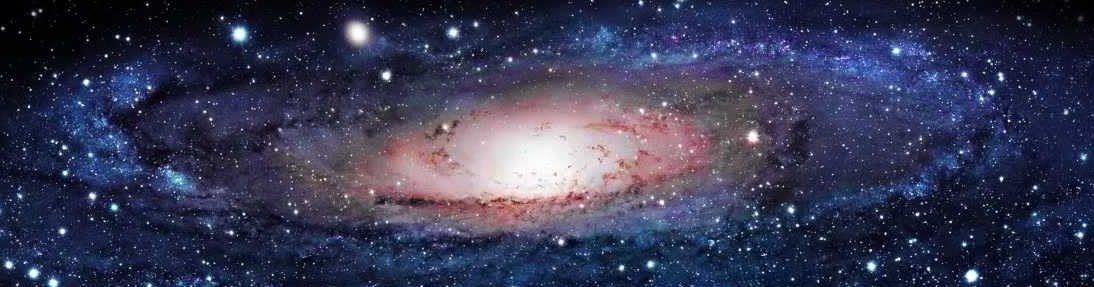
\includegraphics[width=1\linewidth]{../images/astrofooter}
	\caption[Galaxia M88]{Galaxia en espiral \textbf{M88}, a 49 millones de años luz, descubierta por \textbf{Charles Messier} en 1781. \textbf{Fuente:} \cite{M88}}
	\label{fig:astrofooter}
\end{figure}


\subsection{Astronomía en la actualidad}

Viendo el recorrido de esta ciencia en el pasado, nos preguntamos por su repercusión en la sociedad presente. Poniendo en valor los beneficios que tiene su estudio y los interrogantes que a día de hoy científicos de todo el mundo trabajan por dar respuesta \cite{beneficiosastro}.

Los beneficios que obtiene nuestra sociedad, los podemos catalogar según su alcance:

\begin{itemize}
	\item \textbf{Puramente científico}, el impulso por el conocimiento. Responder interrogantes existenciales como: ``¿De dónde venimos?. ¿A dónde vamos?”.


	\item \textbf{La expansión del Universo}, el \textbf{Big Bang}, \textbf{Agujeros Negros}. Conceptos cosmológicos complejos que poco a poco llegan a la sociedad con el esfuerzo de los investigadores a lo largo de décadas, junto con el desarrollo de instrumentos cada vez más sofisticados, para llegar a nuevas conclusiones. 

	\item \textbf{Desarrollo tecnológico}, que posteriormente han tenido aplicaciones directas en la sociedad. Por ejemplo:   \cite{beneficiosastro2}
	
	
	\begin{itemize}
		\item \textbf{Detectores CCD} (\ref{CCD}), que usan nuestras cámaras de fotos fueron inventados en 1969, pero lograron desarrollarse rápidamente gracias a sus aplicaciones en instrumentos astronómicos \cite{ccd}.
		
		\item \textbf{Detectores de rayos X}, que existen en los aeropuertos fueron desarrollados para aplicar los  conocimientos  adquiridos en los detectores de rayos X para instrumentos astronómicos \cite{detectores_rayos_x}.
		
		\item \textbf{Televisión satélite}, con la que estamos familiarizados y usamos a diario en nuestra vida cotidiana \cite{tv_satelite}. 
=======
\bigskip
Los beneficios que obtiene nuestra sociedad los podemos catalogar según su alcance en:
\begin{itemize}
	\item Beneficio puramente científico, el impulso por el conocimiento que ha caracterizado desde siempre al ser humano. Responder interrogantes existenciales como “¿De dónde venimos?, ¿a dónde vamos?”.


	\item Buscar la expansión del Universo, el Big Bang, Agujeros Negros.. son conceptos cosmológicos complejos, que poco a poco  llegan a la sociedad. Para ello ha sido necesario  muchos esfuerzos por parte de investigadores, a lo largo de décadas, junto con el desarrollo de instrumentos cada vez más sofisticados, para llegar a estas conclusiones. 

	\item Desarrollo de numerosas tecnologías que posteriormente han tenido aplicaciones en la sociedad, tenemos varios ejemplos:   \cite{beneficiosastro2}
	
	
	\begin{itemize}
		\item Detectores CCD que usan nuestras cámaras de fotos fueron inventados en 1969, pero lograron desarrollarse rápidamente gracias a sus aplicaciones en instrumentos astronómicos.
		
		\item Detectores de  rayos X que existen en los aeropuertos fueron desarrollados  para aplicar los  conocimientos  adquiridos en los detectores de rayos X para instrumentos astronómicos. 
		
		\item Televisión satélite, con la que estamos familiarizados y usamos a diario en nuestra vida cotidiana. 
		
>>>>>>> c9f08dfe66521d4f0dba18e652f93a6a37a333aa
	\end{itemize}
\end{itemize}


\subsection{Astronomía amateur}

<<<<<<< HEAD
La astronomía \textbf{amateur} es la realizada por astrónomos no profesionales, normalmente sin formación reglada en la materia, y que su interés primordial esta en aprender, conocer esta ciencia, asistir a charlas o quedadas astronómicas y compartir esta afición con otras personas.


La labor de este conjunto es muy valorada, dado que suelen compartir sus trabajos, colaborando con asociaciones y nutriendo de numeroso material muy variopinto: observaciones desde múltiples ubicaciones, momentos en el tiempo o equipo de observación diferente, ampliando así la cantidad de muestras. No puede en este caso llevar más razón el refranero español: \textit{``Más ven cuatro ojos que dos''}.


Todo este trabajo posteriormente puede ser organizado y estudiado por profesionales y para sacar conclusiones valiosas.


Además, muchos astrónomos aficionados, dedican tiempo y energías impartiendo conferencias divulgativas que acercan esta ciencia, sus métodos y sus conclusiones al gran público.


Otro de los perfiles más visuales en el mundo de la astronomía amateur es el de la \textbf{astrofotografía} ~\cite{AstroFoto} (figura~\ref{fig:nightsky}), que consiste en la captación fotográfica de las imágenes de cuerpos celestes, teniendo gran valor artístico en muchos casos.


=======
La astronomía \textbf{amateur} es la realizada por astrónomos no profesionales, normalmente sin realizar formación reglada, y que su interés primordial esta en aprender, conocer esta ciencia, asistir a charlas o quedadas astronómicas y compartir esta afición con otras personas.

\bigskip
La labor de este conjunto es muy valorada, dado que suelen compartir sus trabajos, colaborando con asociaciones  y nutriendo de numeroso material muy variopinto: observaciones desde múltiples ubicaciones, momentos en el tiempo o equipo de observación diferente, ampliando así la cantidad de muestras. No pudiendo llevar más razón el refranero español, \textit``Más ven cuatro ojos que dos"

\bigskip
Todo este trabajo posteriormente puede ser organizado por profesionales y sacar conclusiones.

\bigskip
Tampoco podemos olvidar la labor divulgativa dado que muchos astrónomos aficionados dedican tiempo y energías impartiendo conferencias tanto en agrupaciones, como en actos culturales promovidos por municipios, escuelas o universidades. 

\bigskip
Uno de los perfiles más visuales, es  la \textbf{astrofotografía} ~\cite{AstroFoto}, que consiste  en la captación fotográfica de las imágenes de  cuerpos celestes, teniendo gran valor artístico en muchos casos.

\bigskip
>>>>>>> c9f08dfe66521d4f0dba18e652f93a6a37a333aa
En muchas ocasiones, la frontera entre astrónomos profesionales y amateur es muy tenue porque ambos contribuyen de manera destacada al conocimiento del cielo.


\begin{figure}
\centering
<<<<<<< HEAD
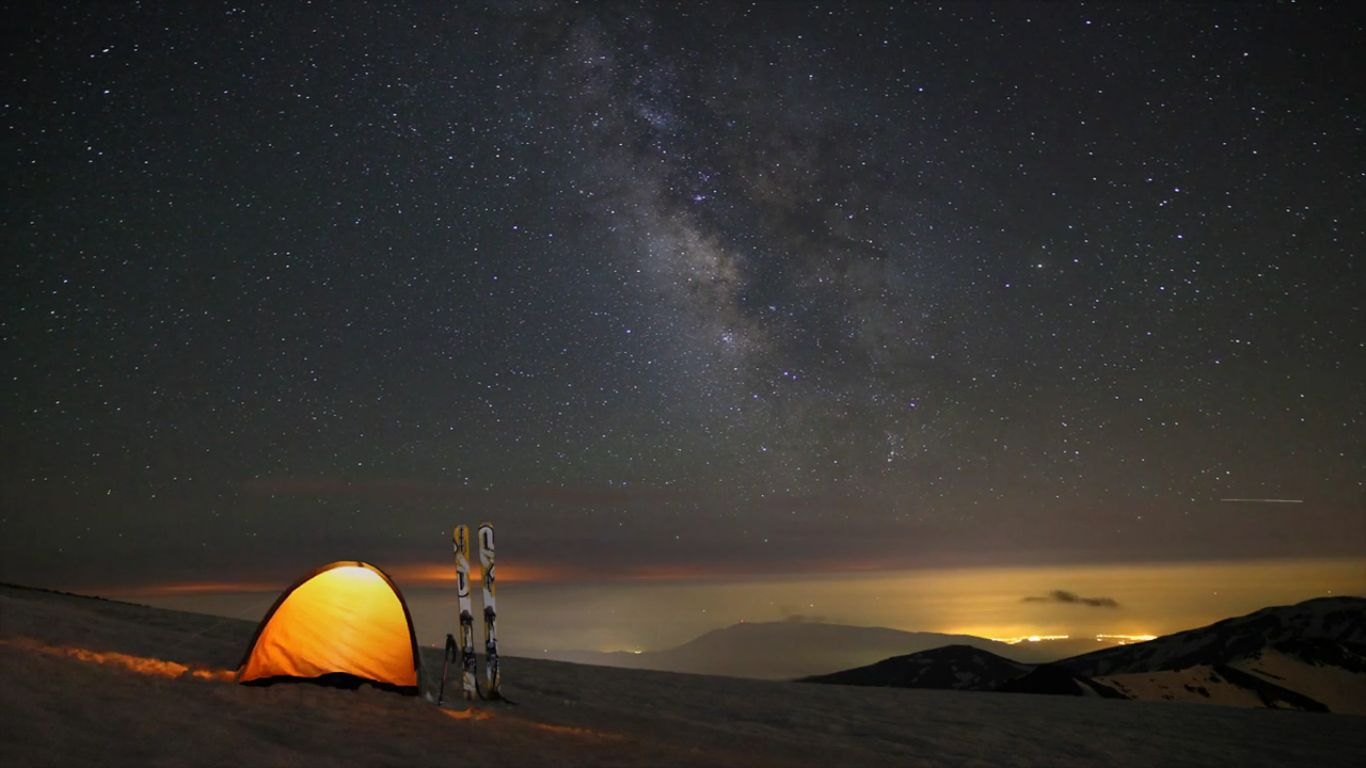
\includegraphics[width=1\linewidth]{../images/nightsky}
\caption[Sierra Nevada Night Sky Time Lapse]{\textbf{Isidro Villo - Sierra Nevada Night Sky Time Lapse}, fotograma del vídeo tomado entre junio y agosto de 2011 en Sierra Nevada en memoria de su compañero Iker Canales Onaindia, muestra el lado más creativo y artístico de la astronomía. \textbf{Fuente:} \cite{sierra_nevada_sky}}
=======
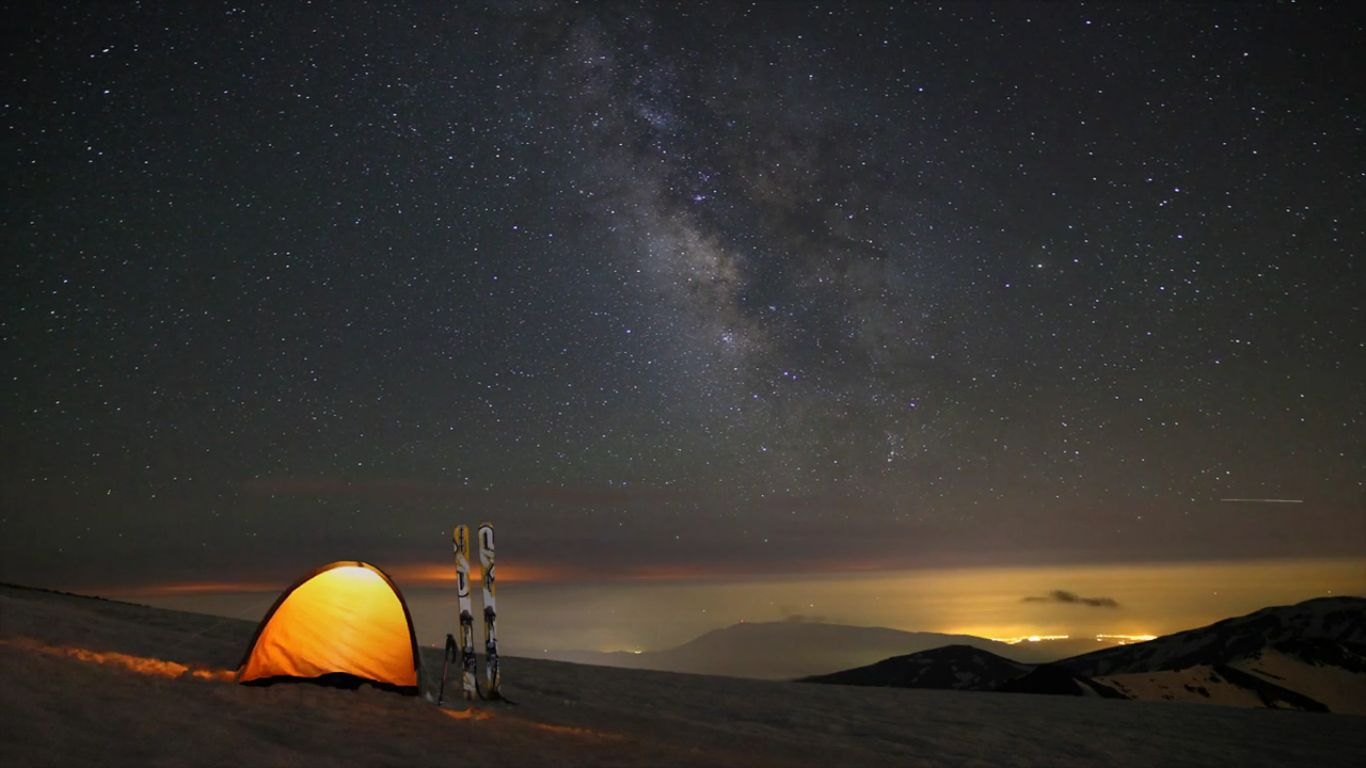
\includegraphics[width=0.7\linewidth]{../images/nightsky}
\caption{\href{https://vimeo.com/28399458}{Isidro Villo - Sierra Nevada Night Sky Time Lapse}}
>>>>>>> c9f08dfe66521d4f0dba18e652f93a6a37a333aa
\label{fig:nightsky}
\end{figure}



\section{Instrumental Astronómico}

<<<<<<< HEAD
La astronomía está intimamente relacionada con una serie de herramientas e instrumentos que permiten expandir los sentidos del observador, permitiendo llegar a ver objetos más lejanos y tenues y apreciar más características de ellos. A continuación se describen algunos de estos instrumentos. 

\subsection{Telescopios} \label{telescopio}
=======
Como ya he enunciado anteriormente la astronomía también está relacionada  con una serie de herramientas e instrumentos básicos que permiten expandir los sentidos del observador, permitiendo llegar a ver objetos más lejanos y apreciar más características de ellos.  
>>>>>>> c9f08dfe66521d4f0dba18e652f93a6a37a333aa

El telescopio es un instrumento que básicamente recoge la mayor cantidad posible de luz emitida por un objeto situado fuera de la atmósfera y la concentrar para así permitir la detección de imágenes que a simple vista son inapreciables \cite{telescopio} (figura~\ref{fig:telescopio}).

<<<<<<< HEAD
=======
El telescopio es un instrumento que básicamente recoge la mayor cantidad posible de luz emitida por un objeto situado fuera de la atmósfera y concentrarla, para así permitir la detección de imágenes que a simple vista son inapreciables\cite{Telescopio}.
>>>>>>> c9f08dfe66521d4f0dba18e652f93a6a37a333aa


\begin{figure}[!ht]
	\begin{center}
		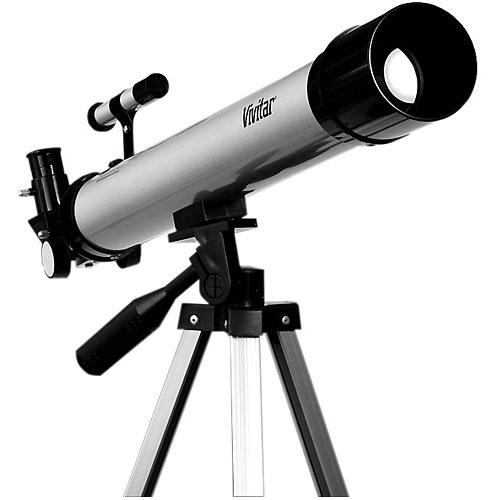
\includegraphics[width=0.6\textwidth]{../images/telescopio2.jpg}
<<<<<<< HEAD
			\caption[Telescopio]{Vista de un telescopio refractor \textbf{Fuente:} \cite{telescopio}}	
		\label{fig:telescopio}
	\end{center}
\end{figure}


 Es una herramienta fundamental en astronomía, y cada mejora de este instrumento ha permitido avances en la comprensión del Universo.

=======
			\caption[Telescopio]{Telescopio \href{http://cienciaaaoa.blogspot.com.es/2014/11/instrumentos-cientificos_20.html}{Telescopio}.}
		\label{fig:telescop}
	\end{center}
\end{figure}

\bigskip
 Es una herramienta fundamental en astronomía, y cada desarrollo o perfeccionamiento de este instrumento ha permitido avances en la comprensión del Universo.
>>>>>>> c9f08dfe66521d4f0dba18e652f93a6a37a333aa

Debemos agradecer este instrumento en gran parte a \textbf{Galileo} \cite{galileo}, cuyos avances permitieron usar el aparato como instrumento astronómico. 

Existen dos grandes tipologías entre los telescopios, según el tipo de sistema óptico que utilizan: los \textbf{reflectores} y los \textbf{refractores}. 


\textbf{Los reflectores} (figura~\ref{fig:reflector}) se constituyen de un espejo principal (espejo primario u objetivo), el cual no es plano como los espejos convencionales, sino que es provisto de cierta curvatura que le permite concentrar la luz en un punto.

\begin{figure}[h]
	\centering
	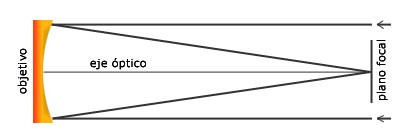
\includegraphics[width=1\linewidth]{../images/refrector}
	\caption[Diagrama telescopio reflector]{Diagrama funcionamiento telescopio reflector \\ \textbf{Fuente:} \cite{tipos_telescopios}}
	\label{fig:reflector}
\end{figure}

<<<<<<< HEAD

\textbf{Los refractores} (figura~\ref{fig:refractor}) poseen como objetivo una lente (o serie de lentes, la cantidad varía según el diseño y calidad) que de forma análoga al funcionamiento de una lupa, concentran la luz en el plano focal. 
=======
Existen varios diseños para este tipo de telescopios. Los mas conocidos entre los aficionados son el \textbf{reflector Newtoniano} y el \textbf{reflector Schmidt-Cassegrain}. 


\bigskip
Los refractores poseen como objetivo una lente (o serie de lentes, la cantidad varía según el diseño y calidad) que de forma análoga al funcionamiento de una lupa, concentran la luz en el plano focal. 
>>>>>>> c9f08dfe66521d4f0dba18e652f93a6a37a333aa


\begin{figure}[h]
	\centering
	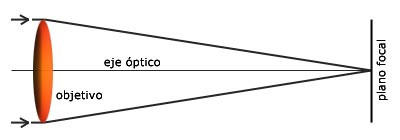
\includegraphics[width=1\linewidth]{../images/refractor}
		\caption[Diagrama telescopio refractor]{Diagrama funcionamiento telescopio Refractor \\ \textbf{Fuente:}\cite{tipos_telescopios} }
	\label{fig:refractor}
\end{figure}



\subsection{Cámaras CCD} \label{ccd}

Un \textit{dispositivo de carga acoplada}, conocido también como \textbf{CCD} (figura~\ref{fig:ccd}) es un circuito integrado que contiene un número determinado de condensadores enlazados bajo el control de un circuito interno. Se encarga de convertir la señal luminosa en una señal eléctrica, componiendo una imagen digital. 


La capacidad de resolución de la imagen, depende del número de células fotoeléctricas del CCD. A mayor número de píxeles, mayor nitidez en relación con el tamaño. Actualmente las cámaras fotográficas digitales incorporan CCD con capacidades de hasta 160 megapíxeles \cite{ccd}.

<<<<<<< HEAD
=======
Dispositivo de carga acoplada (en inglés \textbf{Charge-Coupled Device}, conocido también como \textbf{CCD}), es un circuito integrado que contiene un número determinado de condensadores enlazados bajo el control de un circuito interno. Se encarga de la conversión de una señal luminosa en una señal eléctrica.
>>>>>>> c9f08dfe66521d4f0dba18e652f93a6a37a333aa

\begin{figure}[!ht]
	\begin{center}
		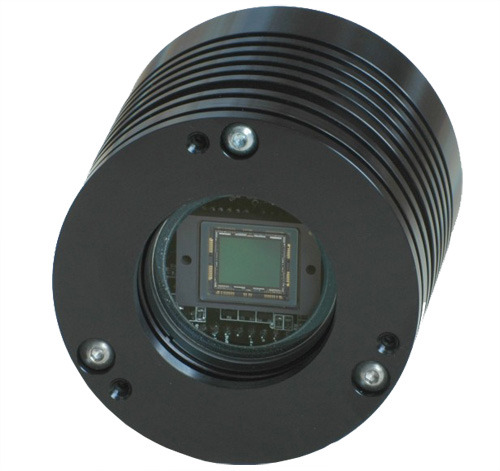
\includegraphics[width=0.6\textwidth]{../images/ccd.jpg}
		\caption[Cámara CCD]{Cámara CCD modelo  Starlight Xpress. \textbf{Fuente:}\cite{ccd_ellunatico}}
		\label{fig:ccd}
	\end{center}
\end{figure}


<<<<<<< HEAD
\subsection{Monturas} \label{montura}

La montura de un telescopio (figura~\ref{fig:montura}) es la parte mecánica que une el trípode o base al instrumento óptico o telescopio. Existen varios tipos de monturas, algunas muy simples, otras mas complejas. Hoy en día son comunes las que tienen correctores electrónicos y dispositivos de localización y seguimiento sofisticados (sistemas \textbf{GOTO}).


\begin{figure}[!ht]
	\begin{center}
		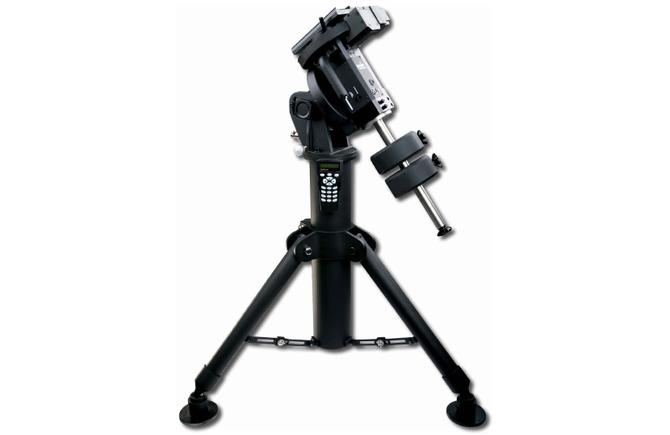
\includegraphics[width=0.8\textwidth]{../images/montura.jpg}
		\caption[Montura]{Montura robotizada modelo SkyWatcher EQ-8  \textbf{Fuente:} \cite{montura_ellunatico}}
		\label{fig:montura}
	\end{center}
\end{figure}

La montura tiene como objetivo proveer de movimiento controlado al telescopio \cite{montura}.


La más simple es la montura \textbf{altacimutal}, que realiza movimientos horizontales y verticales. Este tipo de diseño lo traen incorporados los telescopios pequeños, por lo general \textbf{telescopios refractores} de uso terrestre, dado que su uso es simple, y también varios modelos de equipos automatizados.


Le sigue la \textbf{montura ecuatorial}, que utiliza como plano fundamental el ecuador celeste (proyección del ecuador terrestre). Este diseño usa las coordenadas ecuatoriales, ascensión recta (A.R. o R.A.) y declinación (Dec.), que son proyecciones de las coordenadas terrestres longitud y latitud, respectivamente, sobre la esfera celeste. 


\subsection{Rueda portafiltros} \label{filtros}

La rueda porta-filtros (figura~\ref{fig:portafiltros}), consiste en un cuerpo generalmente de aluminio, que en su interior puede alojar varios \textbf{filtros}. El tamaño de los filtros así como el número de los mismos que puede alojar una rueda portafiltros varía segun los distintos modelos existentes.

Unos filtros comunes son los de colores, utilizados para resaltar las características de los objetos observados, sobre todo la atmosferas y superficies de los planetas.
=======
\bigskip
Físicamente, un \textbf{CCD} es una malla muy empaquetada de electrodos de polisilicio colocados sobre la superficie de un chip. Al impactar los fotones sobre el silicio se generan electrones que pueden guardarse temporalmente. Periódicamente se lee el contenido de cada píxel haciendo que los electrones se desplacen físicamente desde la posición donde se originaron (en la superficie del chip), hacia el amplificador de señal con lo que se genera una corriente eléctrica que será proporcional al número de fotones que llegaron al píxel. Para coordinar los periodos de almacenamiento (tiempo de exposición) y vaciado del píxel (lectura del píxel) debe existir una fuente eléctrica externa que marque el ritmo de almacenamiento-lectura: el reloj del sistema. La forma y amplitud de reloj son críticas en la operación de lectura del contenido de los píxeles.

>>>>>>> c9f08dfe66521d4f0dba18e652f93a6a37a333aa


Gracias a los filtros, podemos fragmentar el espectro de luz dejando pasar luz de una determinada longitud de onda infiriendo a partir de estas mediciones características de los objetos observados.


\begin{figure}[!ht]
	\begin{center}
		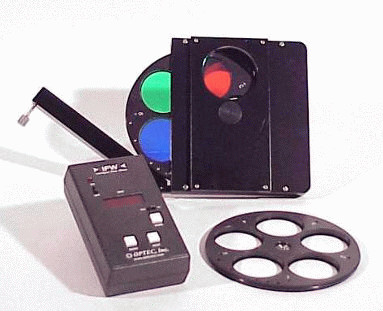
\includegraphics[width=0.6\textwidth]{../images/portafiltros.jpg}
		\caption[Rueda portafiltros]{Rueda portafiltros \textbf{Fuente:} \cite{rueda_portafiltros}).}
		\label{fig:portafiltros}
	\end{center}
\end{figure}


\subsection{Cúpulas}
Las \textbf{cúpulas} (figura~\ref{fig:cupula}) son recintos cerrados mas o menos grandes que nos permiten albergar y proteger el instrumental astronómico. De esta forma, las \textbf{cúpulas} pueden ser abiertas o cerradas para exponer los instrumentos en el momento de las observaciones.


\begin{figure}[!ht]
	\begin{center}
		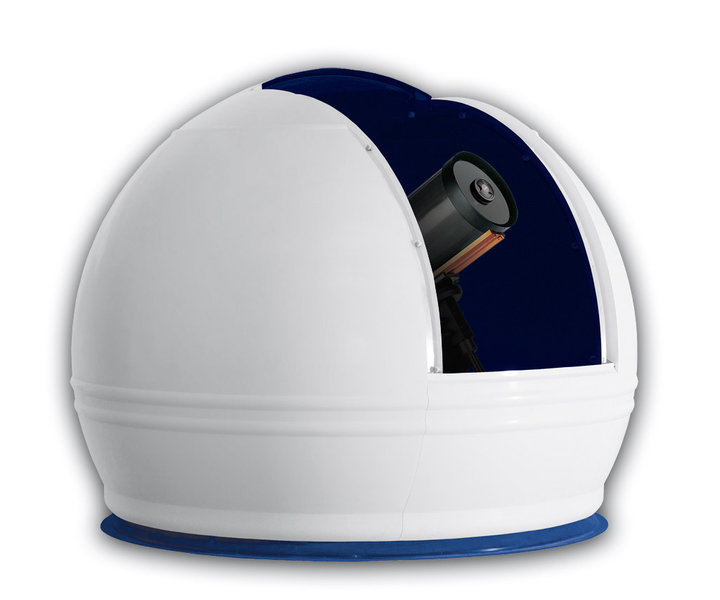
\includegraphics[width=0.65\textwidth]{../images/cupula.jpg}
		\caption[Cúpula]{Cúpula - \textbf{Fuente:} \cite{cupula_ellunatico}.}
		\label{fig:cupula}
	\end{center}
\end{figure}


\subsection{Estaciones meteorológicas} \label{estacion_meteorologica}

Las \textbf{estaciones meteorológicas} son sistemas compuestos por un  un conjunto de sensores que nos proporcionan datos de las distintas magnitudes meteorológicas, tales como la temperatura, humedad, presión barométrica, presencia de nubes, viento, etc... permitiéndonos generar modelos a partir de los cuales conocer la situación climática y su posible evolución. 


Gracias a los datos aportados por las \textbf{estaciones meteorológicas}, podemos conocer la climatología en el momento de realizar observaciones astronómicas. De esta forma podemos decidir si las condiciones son óptimas o si debemos cerrar la cúpula y abortar una observación para evitar daños en los instrumentos por lluvias o similar. 


\subsection{Enfocadores} \label{enfocadores}

El \textbf{enfocador} (figura~\ref{fig:enfocador_tecnosky}), es una pieza fundamental del telescopio que nos permitirá ver con nitidez las imágenes formadas tras la reflexión de la luz en el espejo primario y su desviación por el espejo secundario.


El enfoque viene determinado por la convergencia de la mayor parte de los rayos justo en el plano focal, que es donde colocamos el ojo o una cámara. 


El enfocador, es una pieza adaptada al telescopio, usualmente con una rueda dentada sobre una cremallera que podemos manipular para desplazar el portaocular y variar la distancia focal para encontrar el punto de foco óptimo \cite{enfocador}.


Como en observación astronómica se suele trabajar a muchos aumentos, un pequeño error de enfoque se magnifica en una imagen poco nítida o desenfocada.


Para ayudar en esta operación los astrónomos han perfeccionado algunas técnicas, una de las más extendidas es hacer uso de una \textbf{máscara de enfoque}, \cite{FocusMascara} que consiste en unas rendijas por las que hacemos pasar la luz de un objeto luminoso, difractando los rayos y observando la dirección que toman.


Otra característica que incorporan muchos enfocadores comerciales es la \textbf{compensación por temperatura}, para ello incorpora un sensor térmico en la óptica que informa de oscilaciones en la temperatura (que puedan producir dilatación en la lente o tubo). Cuando se detecta una oscilación considerable en la temperatura, se ejecuta un ciclo de autoenfoque o se compensa según alguna regla establecida.


\begin{figure}[h!]
	\begin{center}
		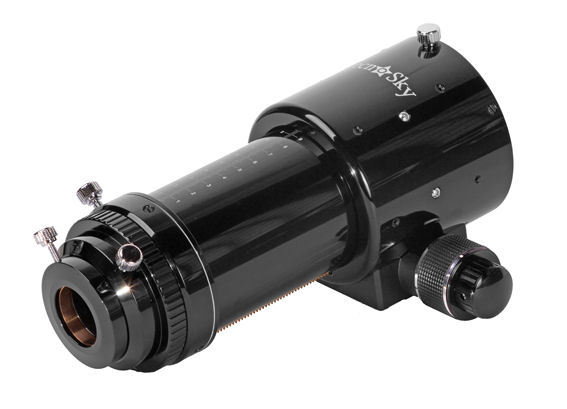
\includegraphics[width=0.6\textwidth]{../images/enfocador.jpg}
		\caption[Enfocador modelo Tecnosky]{Enfocador modelo Tecnosky- \textbf{Fuente:} \cite{enfocador_ellunatico}}
		\label{fig:enfocador_tecnosky}
	\end{center}
\end{figure}


Otra técnica más reciente pero muy extendida entre los astrónomos, es el uso de \textbf{software} especializado, que mediante procesamiento de imagenes es capaz de obtener una medida de la nitidez del objeto observado con el fin de establecer algoritmos automáticos de enfoque.

<<<<<<< HEAD

\section{Software astronómico}

Según su utilidad podemos distinguir y catalogar el software astronómico en los siguientes conjuntos básicos:

\begin{itemize}
	\item \textbf{Planetarios y cartas celestes}: Permiten orientarnos en el cielo, permitiendo así reconocer estrellas, planetas, galaxias, constelaciones. Tiene conexión con bases de datos de todos estos objetos, teniendo información en tiempo real, de su posición. Un ejemplo es \href{http://www.stellarium.org/es/}{\textbf{Stellarium}} \cite{stellarium} o \href{https://www.google.com/intl/es_es/sky/}{\textbf{Google Sky}} \cite{gsky}.
	
	\item \textbf{Alineación y Guiado}: Su función es calibrar y sincronizar los elementos del observatorio (entre ellos y con el movimiento del cielo), para ello también pueden incorporar un ``planetario''. Ejemplos de este tipo de software son \href{https://edu.kde.org/kstars/}{\textbf{KStars}} \cite{kstars} (solución libre) y \href{http://www.cyanogen.com/maxim_main.php}{\textbf{MaxIm DL}} \cite{maximdl}.
	
	\item \textbf{Captura y procesado de imágenes}: se encargan especialmente de capturar imagenes y procesarlas de forma automática. Podemos destacar \href{http://www.mlunsold.com/}{\textbf{ImagesPlus}} (privativo), \href{http://deepskystacker.free.fr/spanish/index.html}{\textbf{Deep Sky Stacker}} y \href{https://github.com/ejeschke/ginga}{\textbf{Ginga}} (software libre) \cite{ginga}. 
	
	
\end{itemize}

\section{Imágenes Astronómicas}

En las imágenes astronómicas interesa almacenar la máxima cantidad de información sobre la imagen, es por ello que siempre se usan formatos \textbf{sin compresión o con compresión sin pérdidas}, como puede ser RAW \cite{Raw} o FITS (figura~\ref{fig:fit}) \cite{FITS}.


\textbf{FITS} es un formato de imágenes especialmente concebido para el mundo de la astronomía, por permitir almacenar información más allá de la visible, así como espectros electromagnéticos.

=======
\bigskip
Para ayudar en esta operación los astrónomos han perfeccionado algunas técnicas, una de las más extendidas es hacer uso de una máscara de enfoque, \cite{FocusMascara} que no es más que unas rendijas por las que hacemos pasar la luz de un objeto luminoso, difractando los rayos y observando la dirección que toman.

\bigskip
Otra característica que incorporan muchos enfocadores comerciales es la \textbf{compensación por temperatura}, para ello incorpora un sensor en la óptica, que informa de  oscilaciones en la temperatura, (que puedan producir dilatación en la lente o tubo), 
cuando se detecta una oscilación considerable en la temperatura, se ejecuta un ciclo de autoenfoque o se compensa según alguna regla establecida.


Una técnica muy extendida entre los astrónomos es el uso de \textbf{software} especializado, que mediante procesamiento de imagenes es capaz de obtener una medida de la nitidez del objeto y compararlo con el valor óptimo.

\bigskip
Dado que es una de los puntos clave del ámbito del proyecto, no paramos a profundizar dado que más adelante enterremos en detalle en la explicación de las medidas, algoritmos, así como las implementaciones de los mismo.


\section{Software astronomico}

\begin{itemize}
	\item \textbf{Planetarios y cartas del cielo}: Permiten orientarnos en el cielo, permitiendo así reconocer estrellas, planetas, galaxias, constelaciones. Tiene conexión con bases de datos de todos estos objetos, teniendo información en tiempo real, de su posición. Un ejemplo es \href{http://www.stellarium.org/es/}{Stellarium} o \href{https://www.google.com/intl/es_es/sky/}{Google Sky}.
	
	\item \textbf{Alineación y Guiado}: Su función es calibrar y sincronizar los elementos del observatorio (entre ellos y con el movimiento del cielo), para ello también pueden incorporar un "planetario". Un ejemplo de tal software es \href{https://edu.kde.org/kstars/}{KStars}, (solución libre) y por \href{http://www.cyanogen.com/maxim_main.php}{MaxIm DL}
	
	\item \textbf{Captura y procesado de imágenes}, se encargan especialmente de capturar imagenes y procesarlas de forma automática, señalar \href{http://www.mlunsold.com/}{ImagesPlus Camera Control} (privativo), \href{http://deepskystacker.free.fr/spanish/index.html}{Deep Sky Stacker} y \href{https://github.com/ejeschke/ginga}{Ginga} (software libre). 
	
	
\end{itemize}

\subsection{Formato imágenes}

En las imagenes astronómicas nos interesa almacenar la máxima cantidad de información sobre la imagen que tomamos, es por ello que siempre se usan formatos sin compresión, como puede ser RAW \cite{Raw} o FITS "Flexible Image Transport System"  \cite{FITS}.

\bigskip
\textbf{FITS} es un formato de imagenes especialmente concebido para el mundo de la astronomía, por permitir almacenar información más allá de la visible, así como espectros electromagnéticos.

\bigskip
Una característica muy interesante para los astrónomos es la incorporación de cabeceras en texto plano y legibles sin software adicional, en esta cabeceras se introducen \textbf{metadatos}, acerca del la observación,  posición geográfica, marcas de tiempo,  características de la cámara, filtros empleados entre otros.

\bigskip
FITS está soportado mediante bibliotecas disponibles en los lenguajes más utilizados en el ámbito científico, incluyendo C, FORTRAN, Java, Perl, PDL, Python, e IDL. 

\begin{figure}[h]
	\centering
	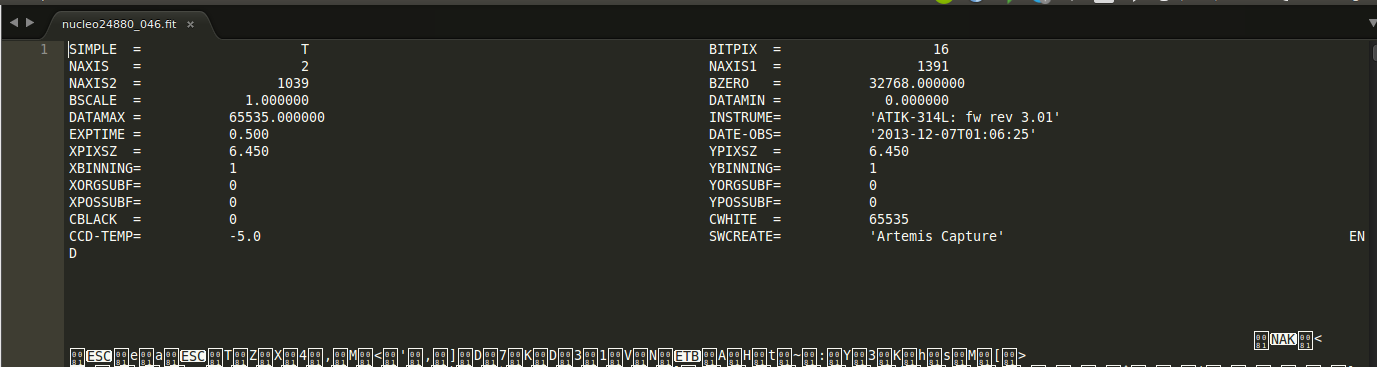
\includegraphics[width=1.0\linewidth]{../images/fit}
	\caption[Cabecera FITS]{Cabecera FITS}
	\label{fig:fit}
	\end{figure}
	
	\bigskip
	Además existen numerosos entornos de procesamiento, que permiten manipular este tipo de imagenes, por nombrar uno de los más conocidos \textbf{ImageJ} \cite{Imagej}.
	
>>>>>>> c9f08dfe66521d4f0dba18e652f93a6a37a333aa

Una característica muy interesante para los astrónomos, es la incorporación de cabeceras en texto plano y legibles sin software adicional: en esta cabecera se introducen \textbf{metadatos} sobre la observación realizada, posición geográfica, marcas de tiempo, características de la cámara, filtros empleados, etc.


<<<<<<< HEAD
FITS está soportado por bibliotecas disponibles en los lenguajes más utilizados en el ámbito científico, incluyendo C, FORTRAN, Java, Perl, PHP, Python.

\begin{figure}[h]
	\centering
	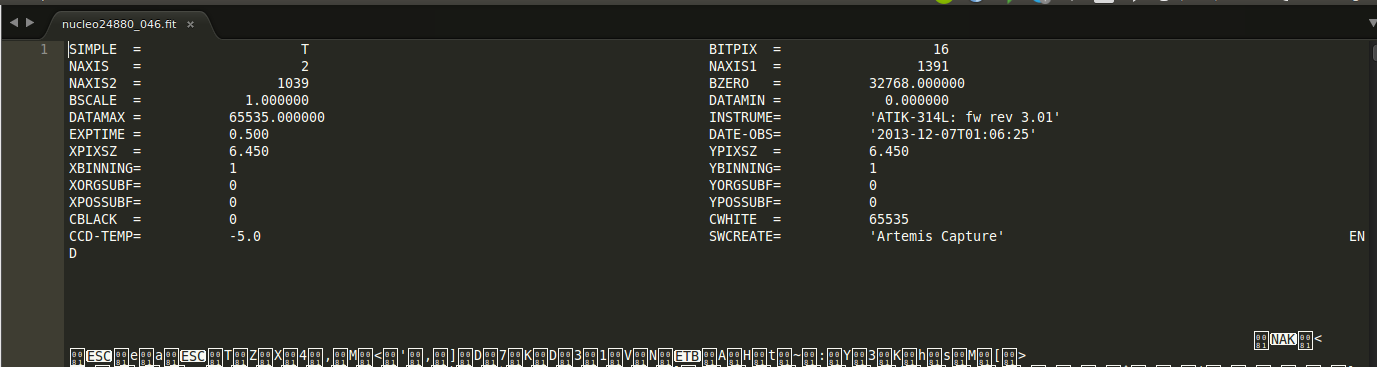
\includegraphics[width=1\linewidth]{../images/fit}
	\caption[Cabecera FITS]{\textbf{Cabecera FITS}. Observamos como se puede leer la cabecera de una imagen en formato FITS usando un editor de texto.}
	\label{fig:fit}
=======
En la actualidad se están implantando diversos protocolos y estándares de manejo remoto al campo de la astronomía, para agilizar y facilitar la observación, librar al astrónomo de tareas tediosas, soportar condiciones climatologías adversas y permitirle centrarse en la propia observación así como multiplicar el numero de puestos, dado que un equipo de astrónomos puede controlar varios observatorios en remoto, mientras que de forma física se ven limitados a uno solo. 

\begin{figure}[h]
\centering
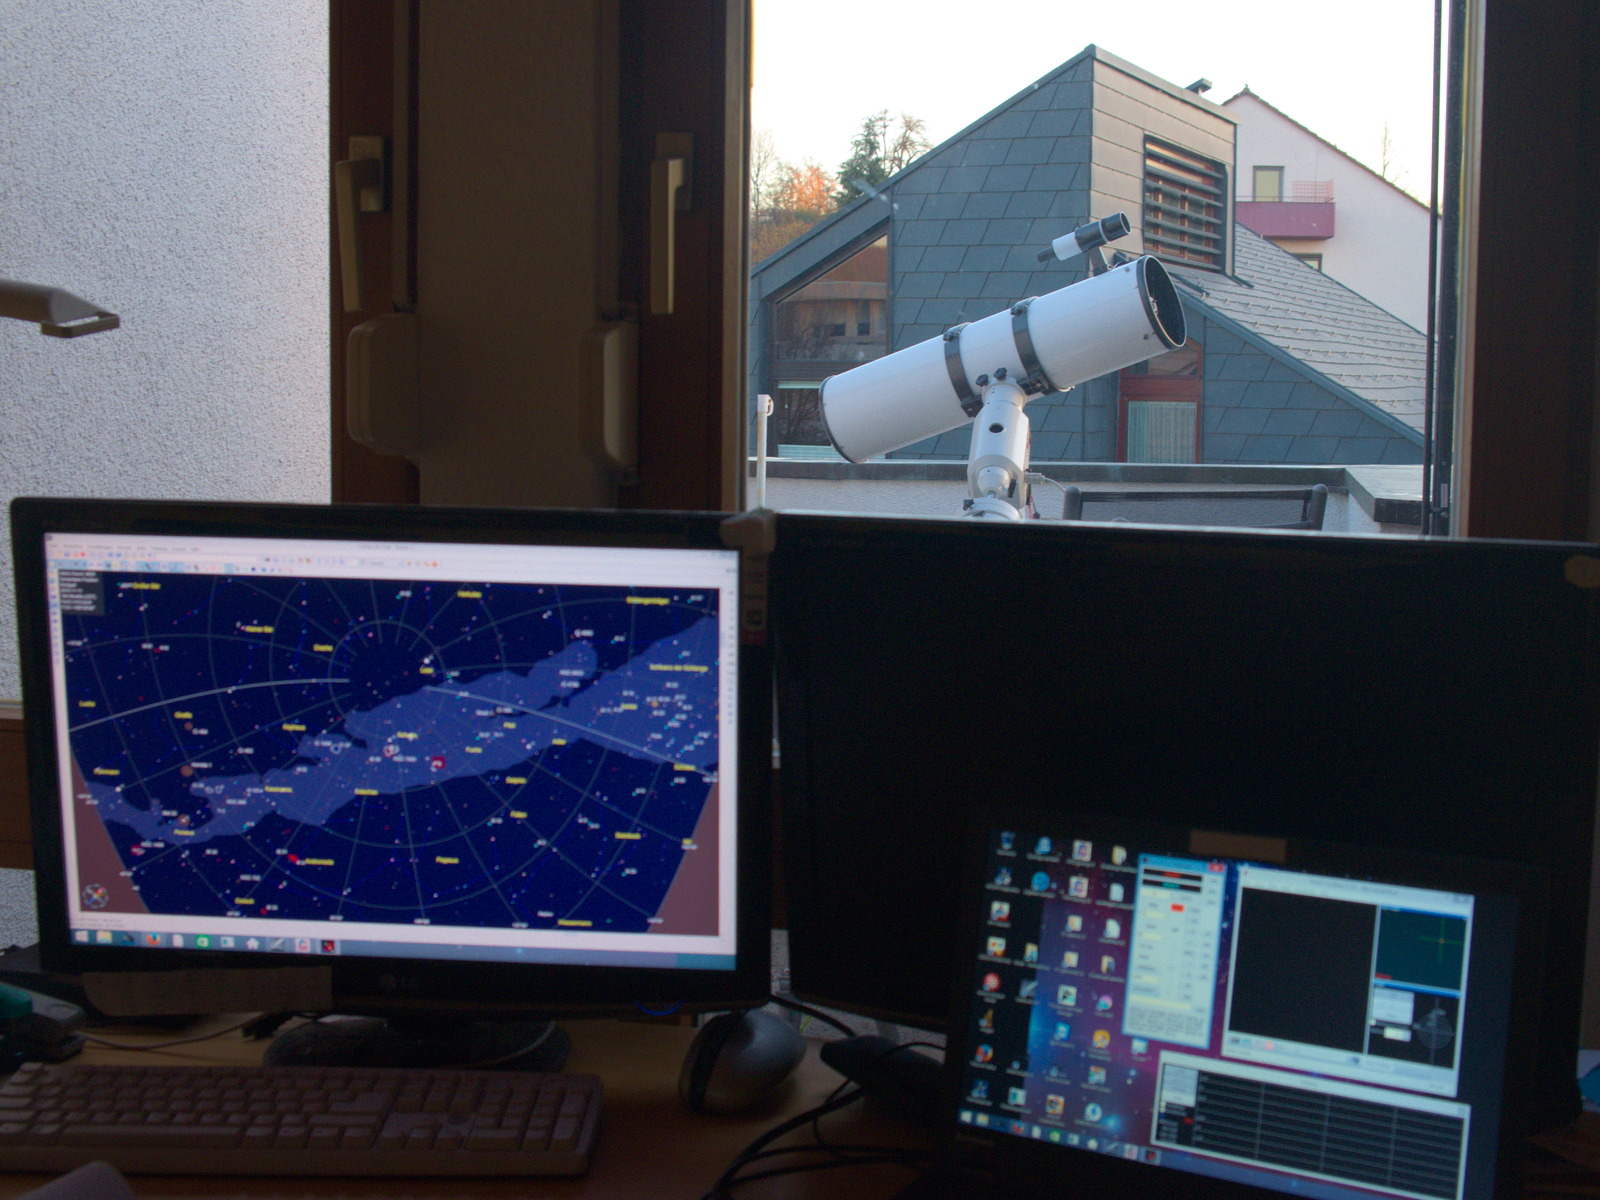
\includegraphics[width=0.7\linewidth]{../images/robotizacion}
\caption{\href{http://www.lost-infinity.com/equipment/}{Observatorio Carsten Schmitt - (Lost Infinity)}}
\label{fig:robotizacion}
>>>>>>> c9f08dfe66521d4f0dba18e652f93a6a37a333aa
\end{figure}
	

Además existen numerosos entornos de procesamiento de imágenes que permiten manipular este tipo de imagenes, como por ejemplo \textbf{ImageJ} \cite{Imagej}.
	

\section{Control remoto de dispositivos astronómicos}

En la actualidad se están implantando diversos protocolos y estándares de control remoto al campo de la astronomía para agilizar y facilitar las observaciones. Estos estándares pretenden librar al astrónomo de tareas tediosas controlar la seguridad en la operación de los instrumentos (por ejemplo condiciones climatologías adversas) y permitirle centrarse en la propia observación, que puede realizarse desde cualquier parte del mundo y a cualquier hora.

También permite multiplicar el número de puestos, dado que un equipo de astrónomos puede controlar varios observatorios en remoto, mientras que de forma física se ven limitados a uno solo. 

Existen diversas formas de controlar los dispositivos astronómicos pero la mayoría presenta los mismos inconvenientes:

\begin{itemize}
	\item Normalmente se controlan los dispositivos diréctamente: conectando cada dispositivo a un PC y se trabaja desde dicho ordenador.
	\item En ocasiones se utilizan herramientas para el control remoto del PCcomo el \textbf{escritorio remoto} \cite{escritorio_remoto}, lo que puede ocasionar algunos inconvenienes como lag excesivo o un consumo de ancho de banda alto.
\end{itemize}

La evolución de las plataformas se puede resumir como sigue:

\begin{enumerate}
<<<<<<< HEAD
\item \textbf{Esquema monolítico:} Cada dispositivo, funciona con \textbf{su propio cliente} y usa un \textbf{protocolo particular}.

\item \textbf{Esquema extensible:} Donde algunos \textbf{fabricantes comparten el código de control}, pero nadie de forma independiente puede implementar nuevos plugins.

\item \textbf{ASCOM}, \ref{ASCOM} intenta crear una \textbf{capa intermedia entre los programas cliente y los dispositivos astronómicos}, dado que es un estándar abierto, cualquiera puede implementar nuevos driver para sus dispositivos. Como inconveniente encontramos que solo puede utilizarse en sistemas \textbf{Microsoft Windows}. Su diseño tiene una relación bastante profunda con el sistema operativo lo cual dificulta el desarrollo basado en red. \cite{ascom}
=======
\item Esquema monolítico:  Cada dispositivo, funciona con us propio cliente y usa su protocolo particular.

\item Esquema extensible: Donde algunos vendedores comparten el código de control, nadie de forma independiente puede implementar nuevos plugins.

\item ASCOM, intenta crear una capa entre los programas para controlar dispositivos astronómicos y los propios dispositivos, dado que es un estándar abierto, cualquiera puede implementar nuevos driver para sus dispositivos, como inconveniente solo puede utilizarse en sistemas \textit{Microsoft Windows}. Su diseño tiene una relación bastante profunda con el sistema operativo lo cual dificulta el desarrollo basado en red.

\item INDI, es más abierto que el anterior y dispone de múltiples implementaciones en C y  Java \cite{indiforjava}, se puede desplegar en en cualquier sistema operativo, ya sea Windows, Linux o Mac. 
>>>>>>> c9f08dfe66521d4f0dba18e652f93a6a37a333aa

\item \textbf{INDI}, es un protocolo \textbf{más abierto que el anterior y dispone de múltiples implementaciones} en C y  Java \cite{indiforjava}, se puede desplegar en cualquier sistema operativo, ya sea \textbf{Windows}, \textbf{Linux} o \textbf{Mac} \cite{indi}. 
\end{enumerate}


\subsection{INDI}

\begin{quote}``\textit{The Instrument Neutral Distributed Interface (INDI) Library is a cross-platform software designed for automation  control of astronomical instruments. It supports a wide variety of telescopes, CCDs, focusers , filter wheels, etc., and it has the capability to support virtually any device. INDI is small, flexible, easy to parse, and scalable. It supports common DCS functions such as remote control, data acquisition, monitoring, and a lot more. With INDI, you have a total transparent control over your instruments so you can get more science with less time.}''
\newline
\\
\textbf{Fuente:} \cite{about_indi}
\end{quote}


El protocolo \textbf{INDI} es una plataforma software diseñada para el control de instrumental astronómico, aunque podría usarse con cualquier dispositivo, incluidos ``virtuales''. La biblioteca \textbf{INDI} permite controlar cualquier dispositivo para el que se haya desarrollado un driver \textbf{INDI}. Funciona mediante el paso de paso de información en formato XML (\ref{XML}). 


Sus principales ventajas frente a otras soluciones para el control de dispositivos son:


\begin{itemize}
	\setlength\itemsep{0.2em}
	\item Es una biblioteca \textbf{ligera}, \textbf{flexible} y \textbf{escalable}.
	\item Es de código abierto por lo que cualquiera puede ver su código y mejorarlo o crear drivers para cualquier dispositivo.
	\item El intercambio de información entre clientes, servidores y drivers es mínimo.
	\item Es \textbf{multiplataforma}.
	\item Separa clara y totalmente el cliente del servidor.
	\item Los fabricantes comienzan a desarrollar drivers para sus dispositivos o liberan las especificaciones para que la comunidad pueda desarrollarlos.
	\item Existen \textbf{numerosos clientes INDI} como \href{https://edu.kde.org/kstars/}{kstars}, \textbf{Cartes Du Ciel}, \textbf{Xephem}, \textbf{Observatorio Remoto} (Android) \cite{obsremoto}, \textbf{Stellarium} \cite{stellarium}.
	
\end{itemize}

<<<<<<< HEAD
\begin{figure}[h]
	\centering
	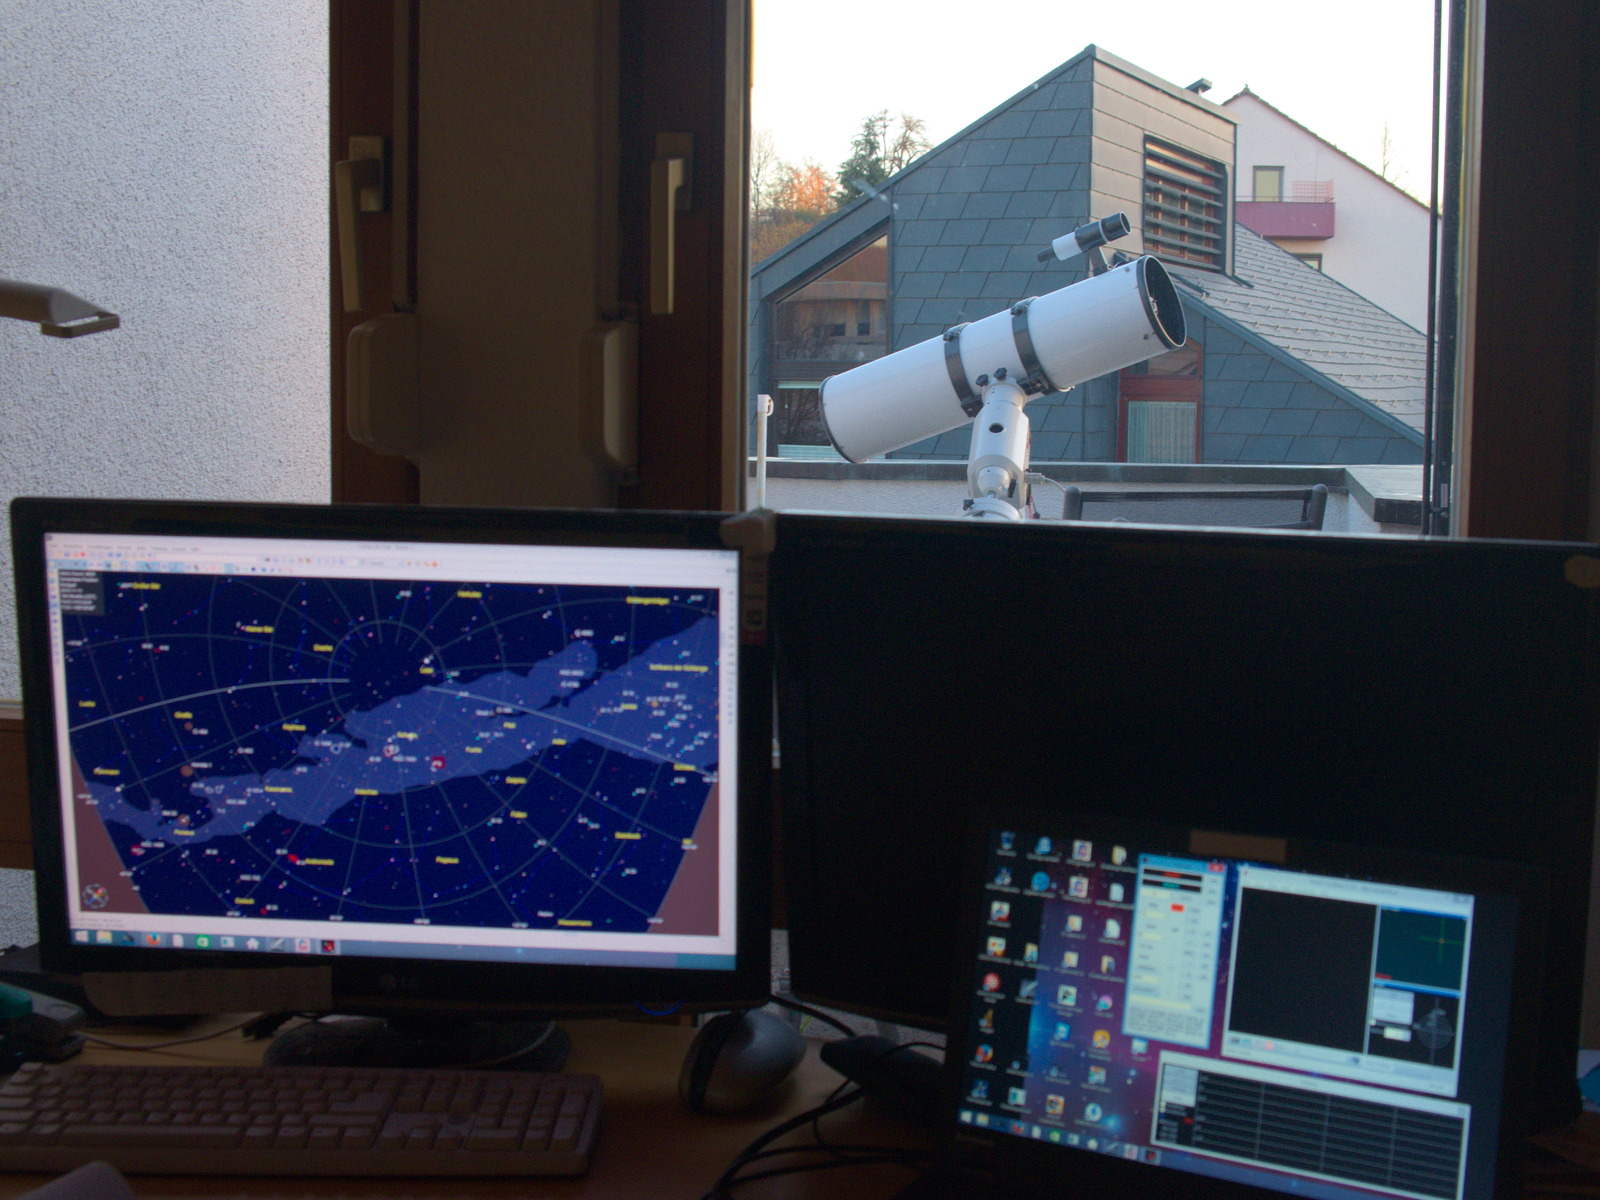
\includegraphics[width=0.9\linewidth]{../images/robotizacion}
	\caption[Observatorio Carsten Schmitt]{Observatorio Carsten Schmitt - (Lost Infinity), haciendo uso de control remoto y software astronómico especializado. \textbf{Fuente:} \cite{lost_infinity}}
	\label{fig:robotizacion}
=======

\bigskip

\subsection{Breve introducción a INDI}

INDI consiste a su nivel más básico en un protocolo que permite el control, automatización, obtención de datos e intercambio de los mismos entre distintos dispositivos hardware y programas cliente. La idea subyacente en el protocolo INDI es desacoplar aspectos específicos del hardware que se controla de tal manera que cambios en el hardware no impliquen necesariamente cambios en el software (cosa que ocurre en sistemas más habituales donde el el frontend software está fuertemente acoplado con el backend hardware.

\bigskip
\begin{figure}[!ht]
	\begin{center}
		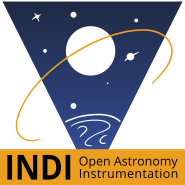
\includegraphics[width=0.21\textwidth]{../images/indi.png}
		\caption[INDI Logo]{INDI Lib (\href{http://indilib.org/}{http://indilib.org/})}
		\label{fig:ascom}
	\end{center}
>>>>>>> c9f08dfe66521d4f0dba18e652f93a6a37a333aa
\end{figure}


\section{Hardware Libre}

Se llama hardware libre a aquellos dispositivos cuyas especificaciones y esquemáticos son de acceso público, ya sea bajo algún tipo de pago, o de forma gratuita. La filosofía del software libre es aplicable a la del hardware libre, y por eso forma parte de la \textbf{cultura libre} \cite{HWLIBRE}.


Los problemas que trata de solventar el hardware libre son los siguientes:

<<<<<<< HEAD
\begin{enumerate}
	\setlength\itemsep{0.2em}
	\item \textbf{Conocimiento restringido}, el conocimiento lo poseen las empresas. El hardware libre trata de hacer pública toda la documentación, diagramas, data shield, fichas, etc.

	\item \textbf{Falta de materiales o herramientas para la fabricación.} 	Tratan de utilizar componentes estándar, que se puedan encontrar fácilmente así como hacer recomendaciones de algunas tiendas online donde puedes comprar tales componentes.  

	\item \textbf{Altos costes de producción.} Al ser de diseño libre, diferentes fábricas pueden ocuparse de proveer los componentes, preocupándose por optimizar y agilizar el proceso, llegando a bajar los costes de producción.

	\item \textbf{Gran inversión en realizar trabajos redundantes.}	No hay que preocuparse por solucionar una y otra vez los mismo problemas: para nuestros diseños podemos partir de otros proyectos consolidados.
\end{enumerate}

=======
Los problemas que trata de solventar el hardware libre:

\bigskip
\begin{enumerate}
	\item Conocimiento lo poseen las empresas.
	Haciendo público todos la documentación, diagramas, data shield, fichas etc.

	\item Falta de materiales o herramientas para la fabricación.
	Tratan de utilizar componentes estándar, que se puedan encontrar fácilmente. 
	Así como hacer recomendaciones de algunas tiendas online donde puedes comprar tales componetes.  

	\item Altos costes de producción.
	Al ser de diseño libre, diferentes factorías pueden ocuparse de fabricar los componentes, preocupandondose por optimizar y agilizar el proceso, llegando a bajar los costes de producción.

	\item Gran inversión en realizar trabajos redundantes. 
	No hay que preocuparse por solucionar una y otra vez los mismo problemas, para nuestros diseños podemos partir de otros proyectos consolidados.
		  
\end{enumerate}
>>>>>>> c9f08dfe66521d4f0dba18e652f93a6a37a333aa

Al auspicio de este movimiento han surgido muchísimas plataformas y tecnologías, pero en especial cabe remarcar dos de las más importantes, \textbf{Arduino} \cite{ARDUINO} y \textbf{Raspberry Pi} \cite{raspberry}.

<<<<<<< HEAD
=======
Dado este movimiento han surgido muchísimas plataformas, pero en especial cabe remarcar dos de las más importantes, Arduino y Raspberry Pi.
>>>>>>> c9f08dfe66521d4f0dba18e652f93a6a37a333aa

\subsection{Arduino}


\begin{figure}
\centering

\includegraphics[width=0.75\linewidth]{../images/arduino}
\caption[Arduino]{Logo oficial de Arduino - \textbf{Fuente:} \cite{ARDUINO}}
\label{fig:arduino}
\end{figure}


<<<<<<< HEAD
\paragraph{Arduino} es una compañía de hardware libre, la cual desarrolla placas de desarrollo (figura~\ref{fig:arduinocasero}) que integran un \textbf{microcontrolador} y un entorno de desarrollo \cite{IDE}.
=======
\bigskip
\paragraph{Arduino} es una compañía de hardware libre, la cual desarrolla placas de desarrollo que integran un \textbf{microcontrolador} y un entorno de desarrollo  \cite{IDE}.

\bigskip
Está diseñado para facilitar el uso de la electrónica en proyectos multidisciplinarios\cite{ARDUINO}.

\bigskip
La primer placa Arduino fue introducida en el 2005, ofreciendo un bajo costo y facilidad de uso para novatos y profesionales buscando desarrollar proyectos interactivos con su entorno mediante actuadores y sensores.
>>>>>>> c9f08dfe66521d4f0dba18e652f93a6a37a333aa

Está diseñado para facilitar el uso de la electrónica en proyectos multidisciplinares \cite{ARDUINO}.

Tal como marcan los principios del hardware libre, los esquemáticos de diseño del Hardware, están disponibles bajo licencia Libre, permitiendo a cualquier persona crear su propia placa Arduino sin necesidad de comprar una prefabricada. 


\begin{figure}[h]
	\centering
	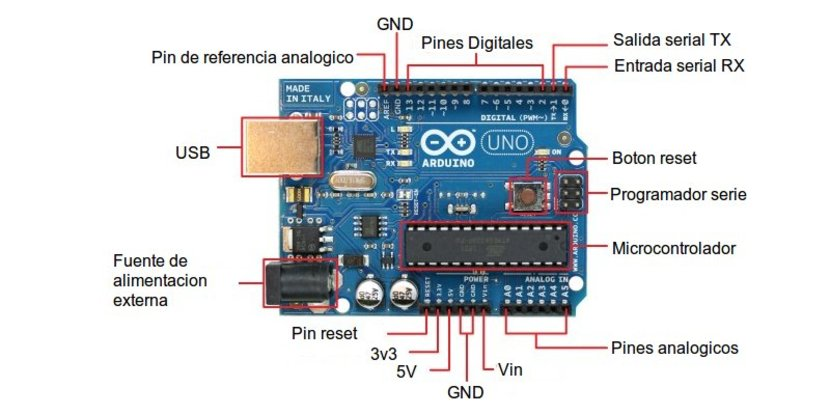
\includegraphics[width=1\linewidth]{../images/caracteristicas_arduino}
	\caption[Diagrama Arduino]{Vista principal placa Arduino, podemos diferencias los diferentes componentes. \textbf{Fuente:} \cite{ARDUINO}}
	\label{fig:arduinocasero}
\end{figure}


\paragraph{Modelos de Arduino}  

Existen multitud de ediciones o modelos de placa, cada una pensada para un público concreto o para una serie de tareas o proyectos específicos. También han surgido muchos modelos no oficiales. 


Por nombrar algunas placas de las más famosas:
\begin{itemize}
\setlength\itemsep{0.2em}	
	
\item \textbf{Arduino UNO}: es la plataforma más extendida y la primera que salió al mercado.

\item \textbf{Arduino Yun}: Combina un chip ATmega32u4 y en un chip Atheros AR9331, que se comunican mediante un puente. El chip Atheros soporta distribuciones ligeras de Linux. 

\item \textbf{Arduino Mega}: Incorpora un chip ATmega2560, dando más rendimiento que el ATmega320 del Arduino UNO

\item \textbf{Arduino Ethernet}: Idéntico al Arduino UNO, pero con conexión a red.

\item \textbf{Arduino Nano y Micro y TinyDuino}: De muy pequeño tamaño y optimizadas para mejorar el consumo. 

\item \textbf{Arduino LilyPad}: está pensado para insertarse en prendas y textiles, es lavable. 

\end{itemize}


\paragraph{Shields para Arduino} 

Son placas de circuitos modulares que se montan unas encima de otras para dar funcionalidad extra a las placas de Arduino.

Las shields, se comunican con Arduino usando algunos de los pines digitales/analógicos, por algún bus como el SPI \ref{SPI}, I2C \ref{I2C} o bien por puerto serie. Además estas shields se alimentan generalmente a través del Arduino mediante los pines de 5V y GND \cite{shield}.

<<<<<<< HEAD
Podemos destacar algunos de los shield más comunes y recomendables para multitud de proyectos:
\begin{itemize}
 \item \textbf{Arduino Wifi Shield}, que añade comunicación wireless WIFI, 
 \item \textbf{Arduino GSM Shield}, comunicación GPRS (usando una tarjeta SIM),
 \item \textbf{Arduino Motor Shield}, permite manejar motores DC,
 \item \textbf{GPS Shield}, añade localización GPS,
 \item \textbf{Xbee Shield}, comunicación inalámbrica XBee \cite{XBee}, entre muchos otros. 
\end{itemize}
   
=======
\bigskip
Las shields se pueden comunicar con el arduino bien por algunos de los pines digitales o analógicos o bien por algún bus como el SPI, I2C o puerto serie, así como usar algunos pines como interrupción. Además estas shields se alimenta generalmente a través del Arduino mediante los pines de 5V y GND\cite{shield}.
>>>>>>> c9f08dfe66521d4f0dba18e652f93a6a37a333aa



\paragraph{Framework desarrollo Arduino}

El lenguaje de programación de Arduino (basado en Wiring) está implementado en C++. Posee su propio entorno de programación (figura~\ref{fig:arduinoide}), con opciones para compilar y cargar el código fuente en la placa que tenemos conectada. Los programas de Arduino se llaman ``sketch'' \cite{arduino_sketch}.

\begin{figure}
\centering
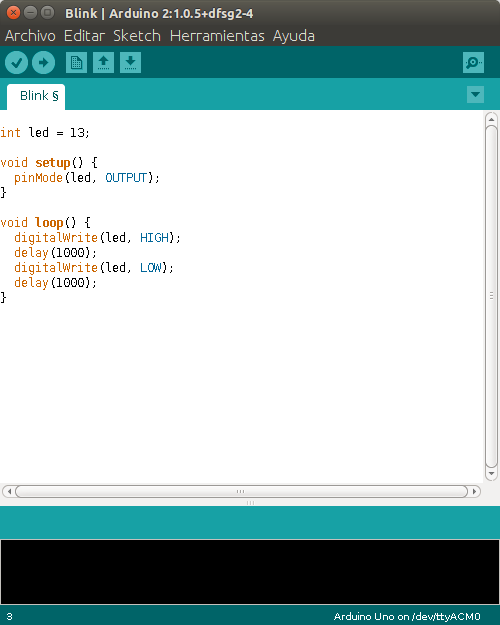
\includegraphics[width=0.9\linewidth]{../images/arduinoide}
\caption[Interfaz de programación de Arduino]{Interfaz de programación de Arduino, con un \textbf{sketch} básico \\ ``Hola Mundo" }
\label{fig:arduinoide}
\end{figure}


También podemos encontrar multitud de bibliotecas y módulos implementados por terceros \cite{arduino_libraries}, que se pueden incorporar directamente a nuestros proyectos, realizando algunas abstracciones sobre el hardware, comunicación o algún aspecto de más bajo nivel.




\subsection{Raspberry Pi}


Raspberry Pi \cite{raspberry} fue lanzado en 2006 por la Fundación Raspberry Pi con el objeto de facilitar la formación de informática en las escuelas de todo el mundo, especialmente en los lugares más desfavorecidos.

Esta placa (figura~\ref{fig:raspberry_pi}), a diferencia que Arduino, es capaz de ejecutar un sistema operativo completo, incluyendo el correspondiente servidor gráfico y servicios básicos como SSH o FTP. 

Actualmente contamos con la versión 3, que incorpora un procesador ARM de 4 núcleos con una velocidad de 1.2 GHz. El otro punto destacable es su GPU, capaz de llegar a resoluciones Full HD sin problema alguno. Junto a las características anteriores, cabe destacar 1 GB de memoria RAM, que permite ejecutar varias aplicaciones al mismo tiempo.

Otro punto a destacar de la Raspberry Pi es su conectividad, ya que incorpora en la misma placa el hardware necesario para dotar al sistema tanto de \textbf{Bluetooth}, de \textbf{WiFi} o de \textbf{Ethernet}.

También puede usarse para prototipado, por lo que incorpora 40 pines \textbf{GPIO} a los que se les puede conectar cualquier dispositivo sensor o actuador.

Recientemente ha aparecido una placa de la misma serie pero de reducidas dimensiones, solo 6x3 cm, a diferencia de la anterior tiene una potencia inferior y no cuenta con módulo de conexión a red.

Por su reducido coste y consumo estas plataformas son ideales para ejecutar servicios básicos, convertirse en concentradores de los datos que proporciona una red de sensores y dar acceso a ellos mediante Internet (función de puerta de acces o gateway).



\begin{figure}[h]
\centering
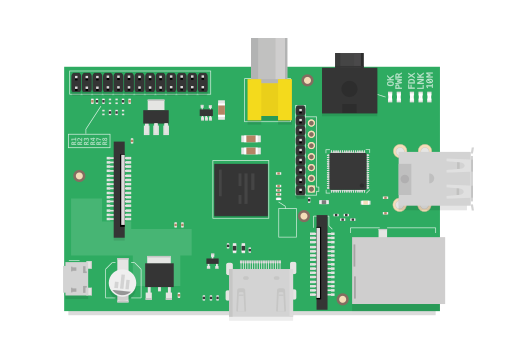
\includegraphics[width=0.8\linewidth]{../images/raspberry_pi}
\caption[Raspbery Pi]{Raspbery Pi \textbf{Fuente:} \cite{imagen_raspberrypi}}
\label{fig:raspberry_pi}
\end{figure}




\section{Enfocadores astronómicos: estado del arte}

Entendemos estado del arte como aquellos desarrollos de última tecnología realizados sobre un producto, que han sido probados en la industria y han sido acogidos y aceptados por diferentes fabricantes.

Dado el alcance e interés de este proyecto es de obligado cumplimiento el hacer una investigación entre los diferentes fabricantes de la soluciones existentes para el enfoque automático en astronomía. Una búsqueda en Internet nos ofrece algunas alternativas:

\begin{itemize}
	\item \textbf{Orion AccuFocus} \cite{orion_focuser}: Muy básico: ni control por ordendor, ni pantalla, ni botones de control preciso. Tiene un precio en el mercado de 99\$. 
	\item \textbf{FocusMaster} \cite{focusmate}, cuenta con las funciones básicas de control, incluido ajuste de velocidad y ajuste de movimiento fino. Su precio oscila en torno a los 200\$.  
	\item \textbf{Opetec} es uno de los fabricantes más especializados y dispone de varios modelos, el más económico tiene un precio de 725\$.
	\item \textbf{Robofocus}, una de las soluciones más avanzadas y extendidas, tiene un precio de 495\$.
\end{itemize}

A continuación detallamos un poco más las soluciones existentes más populares y completas.

\subsection{Opetec}

\textbf{Opetec} es uno de los fabricantes más importantes en el mundo de los productos electro-ópticos usados en astronomía. Su sede central se localiza en Lowell (Michigan, EEUU).

<<<<<<< HEAD

Entre los productos más económicos para enfoque astronómico contamos con el modelo, \textbf{17670 - Original TCF-S} (figura~\ref{fig:optecinc_focuser}), cuyas características estrellas son la \textbf{compensación térmica} y un \textbf{backlash pequeño}.


=======
>>>>>>> c9f08dfe66521d4f0dba18e652f93a6a37a333aa

\begin{figure}[h]
\centering
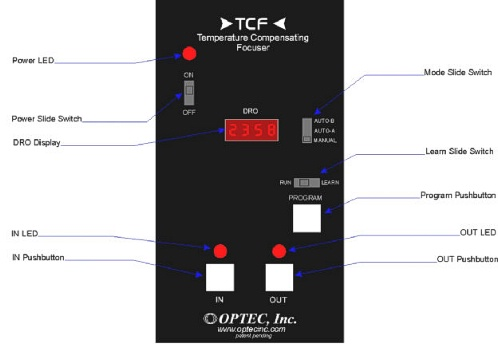
\includegraphics[width=0.9\linewidth]{../images/optecinc_focuser}
\caption[Opetec Original TCF-S]{Mando de control Opetec Original TCF-S. \textbf{Fuente:} \cite{optec}}
\label{fig:optecinc_focuser}
\end{figure}

<<<<<<< HEAD

La misma compañía cuenta con un software especifico para corregir el foco en tiempo real,\textbf{FocusLock Focusing Software} (figura~\ref{fig:focus_lock}).

\begin{figure}[h]
\centering
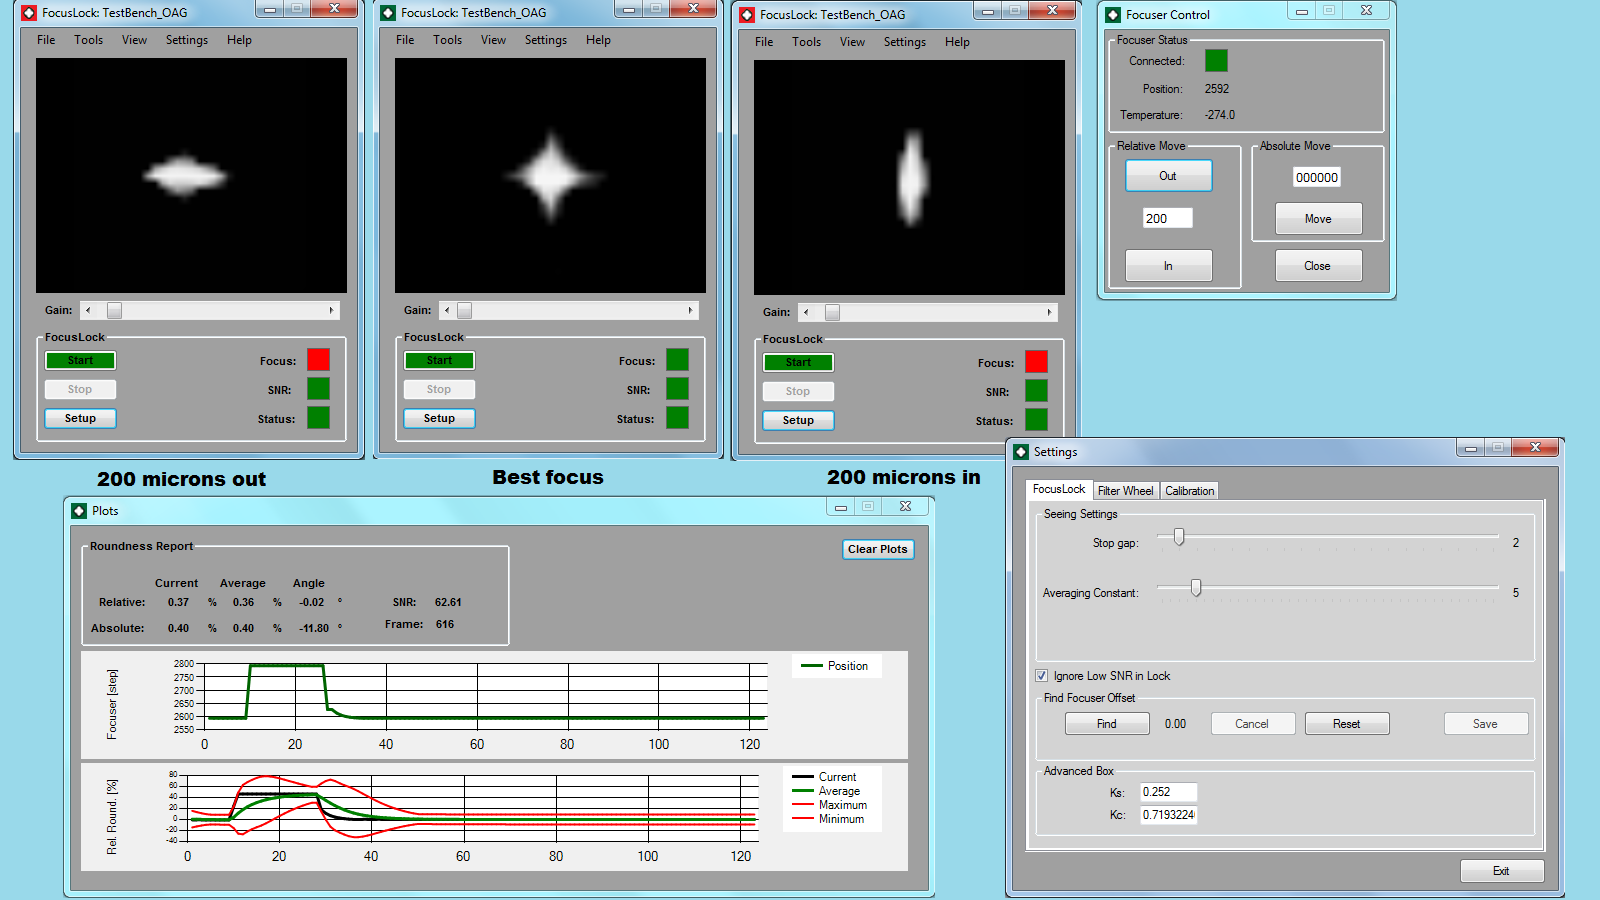
\includegraphics[width=1\linewidth]{../images/focus_lock}
\caption[Opetec Focus Lock]{Software Opetec Focus Lock en un ciclo de funcionamiento \textbf{Fuente:} \cite{optec} }
\label{fig:focus_lock}
\end{figure}

Se trata de un producto de alta calidad, pero su precio es elevado y el software requiere de la plataforma \textbf{ASCOM} (\ref{ASCOM}) lo que limita su uso. 



\subsection{Robofocus}
\label{sec:robofocus}

Robofocus (figura~\ref{fig:robofocus2}) es uno de los enfocadores astronómicos más populares que existen en el mercado es \textbf{Robofocus} \cite{robofocus}.

\begin{figure}
\centering
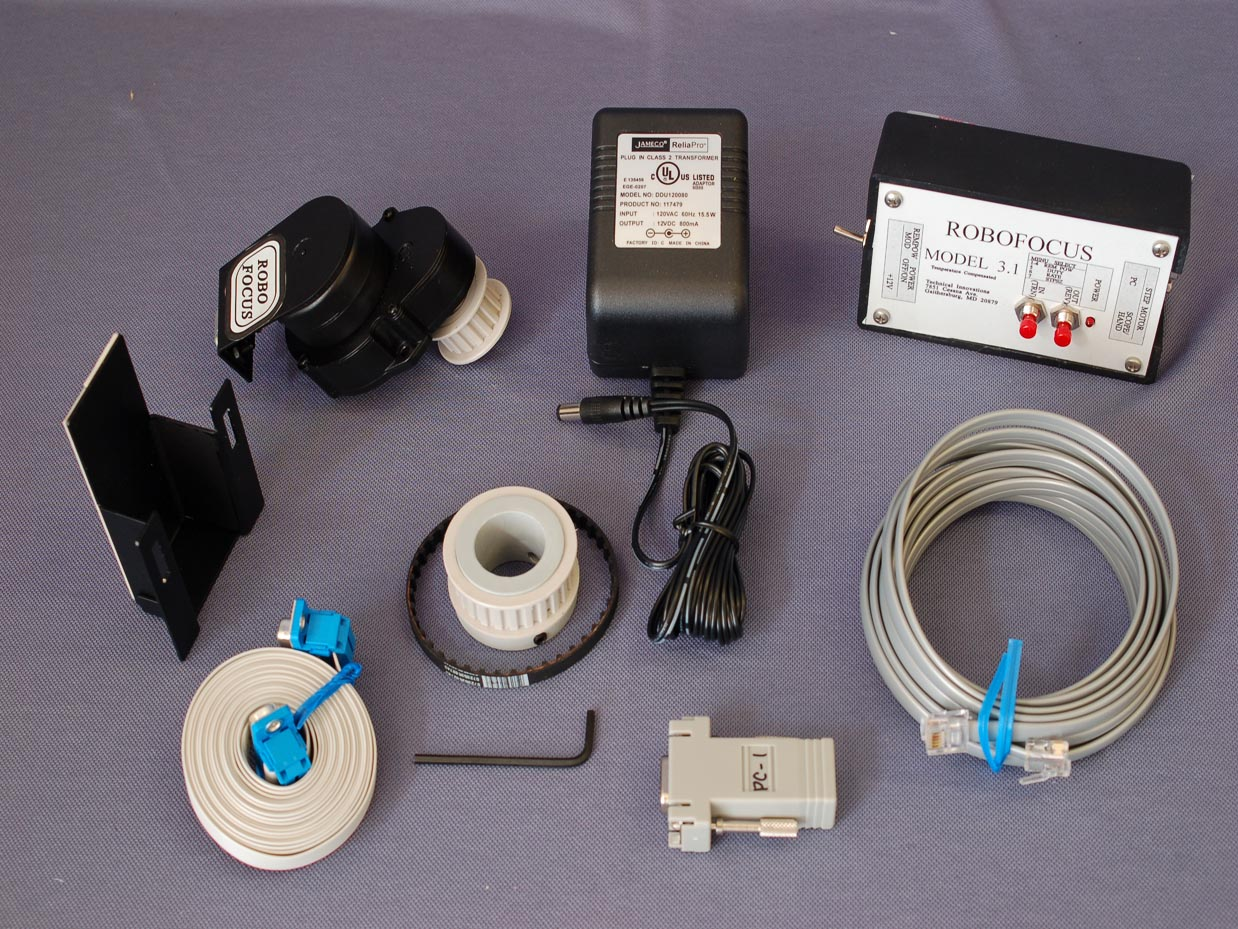
\includegraphics[width=1\linewidth]{../images/robofocus2}
\caption[Kit Robofocus]{Componentes de un kit Robofocus. \textbf{Fuente:} \cite{robofocus}}
\label{fig:robofocus2}
\end{figure}

Además una de contar con todas las características anteriores de la solución ofrecida por Opetec, incluida la componesación por cambio de temperatura, Robofocus es compatible con la plataforma INDI \cite{robofocus_indi}. 

Investigando el funcionamiento del dispositivo se puede encontrar el protocolo serie (tabla~\ref{robofocus_command}) que utiliza, que utiliza el siguiente formato:

\begin{itemize}
	\item \textbf{F} : Indica que es un comando del enfocador.
	\item \textbf{X} : Caracter alpha, selecciona el comando.
	\item \textbf{?} : Separador
	\item \textbf{NNNNNN} : Seis caracteres decimales (completando con ceros sí es necesario).
	\item \textbf{Z} : Checksum, suma de verificación del comando. 
\end{itemize}





\begin{table}[h]
	\centering
	\caption[Comandos Robofocus]{Descripción de los comandos de Robofocus}
	\label{robofocus_command}
	\begin{tabular}{|l|l|l|}
		\hline
		Comando   & Parámetro             & Descripción                                                                                   \\ \hline\hline
		FV      & -         & Consulta versión del firmware.                                                                              \\ \hline
		FG      & XXXXX     & Mueve a posición.                                                                                           \\ \hline
		FI      & XXXXX     & Mueve X pasos hacia el interior.                                                                            \\ \hline
		FO      & XXXXX     & Mueve X pasos hacia el exterior.                                                                            \\ \hline
		FS      & XXXXX     & Asigna posición actual como posición X.                                                                     \\ \hline
		FL      & XXXXX     & Asigna máximo recorrido.                                                                                    \\ \hline
		FP      & XXXXX     & \begin{tabular}[c]{@{}l@{}}Activa salidas de corriente electrica adicional, \\ para alimentar dispositivo adicional.\end{tabular} \\ \hline
		FB      & NXXXXXZ   & Cambia la compensación de backlash.                                                                         \\ \hline
		FT      & -         & Responde con la temperatura.   \\ \hline     
	\end{tabular}
\end{table}


A la vista de lo presentado podemos concluir que pese a que existen diversas soluciones para control del foco en astronomía, dichas soluciones:

\begin{itemize}
 \item Son privativas (lo que dificulta su mejora, estudio, modificación o arreglo).
 \item Solo funcionan bajo la plataforma ASCOM (Windows).
 \item Son caras (para lo que ofrecen).
\end{itemize}

Estos motivos son los que llevan a pensar que el desarrollo de una solución completa de enfoque que sea libre es algo interesante y que puede tener una cierta apreciación por los astrónomos (sobretodo los amateur).


=======
>>>>>>> c9f08dfe66521d4f0dba18e652f93a6a37a333aa
